%% \chapter[htoc-titlei][hhead-titlei]{htitlei}
%% -----------------------------------------------------------------------------
\chapter[Signal model interpretation][Signal model interpretation]
        {Signal model interpretation}
\label{sec:axp_interpretation_plots}

%% -----------------------------------------------------------------------------
This appendix includes plots of the expected and observed $CL_S$ values in each
of the two SRs.
The $CL_S$ values are computed for each of the tested stop masses from 400~\GeV
to 1100~\GeV, and over the range of physical stop branching ratios.
In addition to the $CL_S$ values, the selected SR for a selection of stop
branching ratios is shown for each stop mass.
The SR is selected by choosing the SR which gives the lowest expected $CL_S$
value for the particular choice of stop mass and branching ratios as described
in Section~\ref{sec:model_dependent_limits}

%% -----------------------------------------------------------------------------
\newpage
\section{400 \texorpdfstring{\GeV}{GeV} stop mass}

\begin{figure}[ht]
  \centering
  \subbottom[Expected $CL_S$ or SR~400]{
    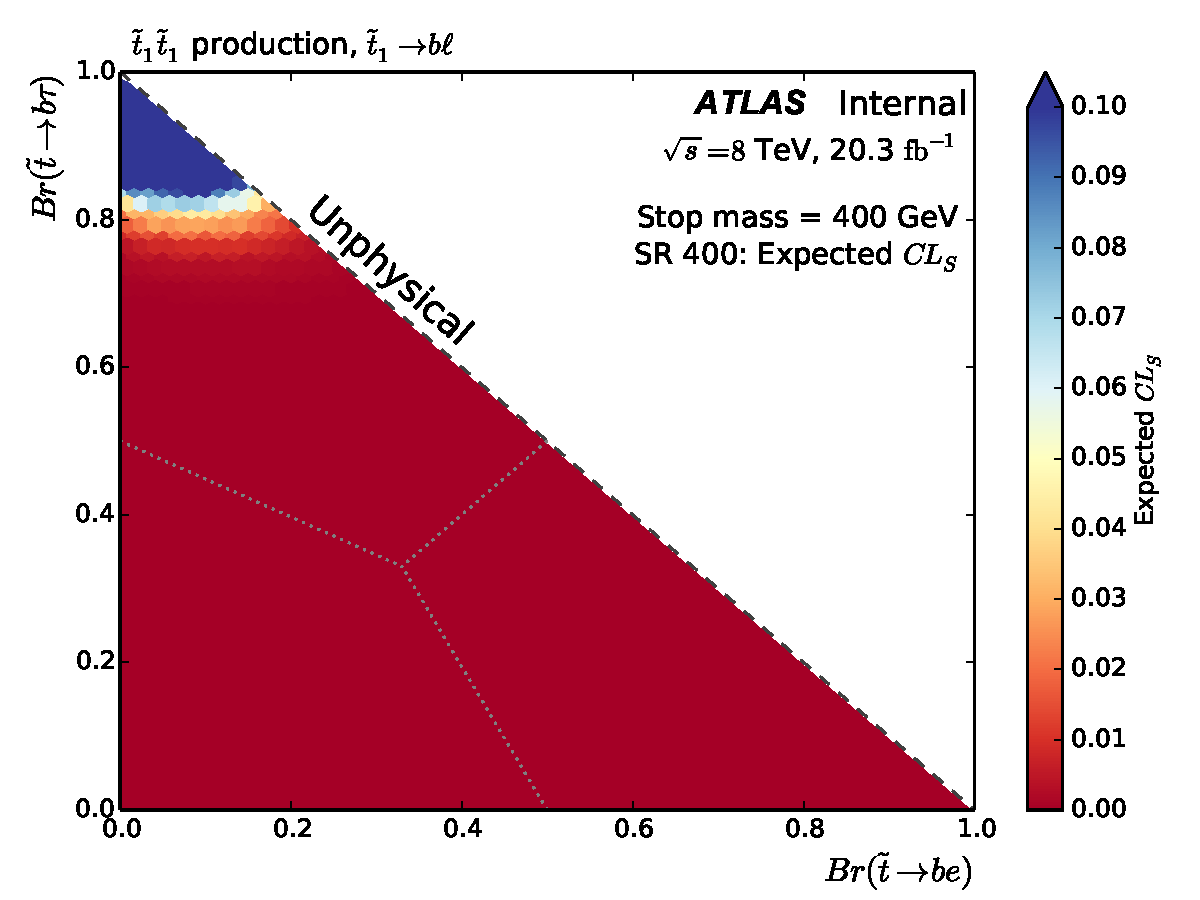
\includegraphics[width=0.65\textwidth]
      {figs/blstop/cls_plots/cls_vs_br_m_400_sr_400_exp.pdf}
  }
  \subbottom[Expected $CL_S$ or SR~600]{
    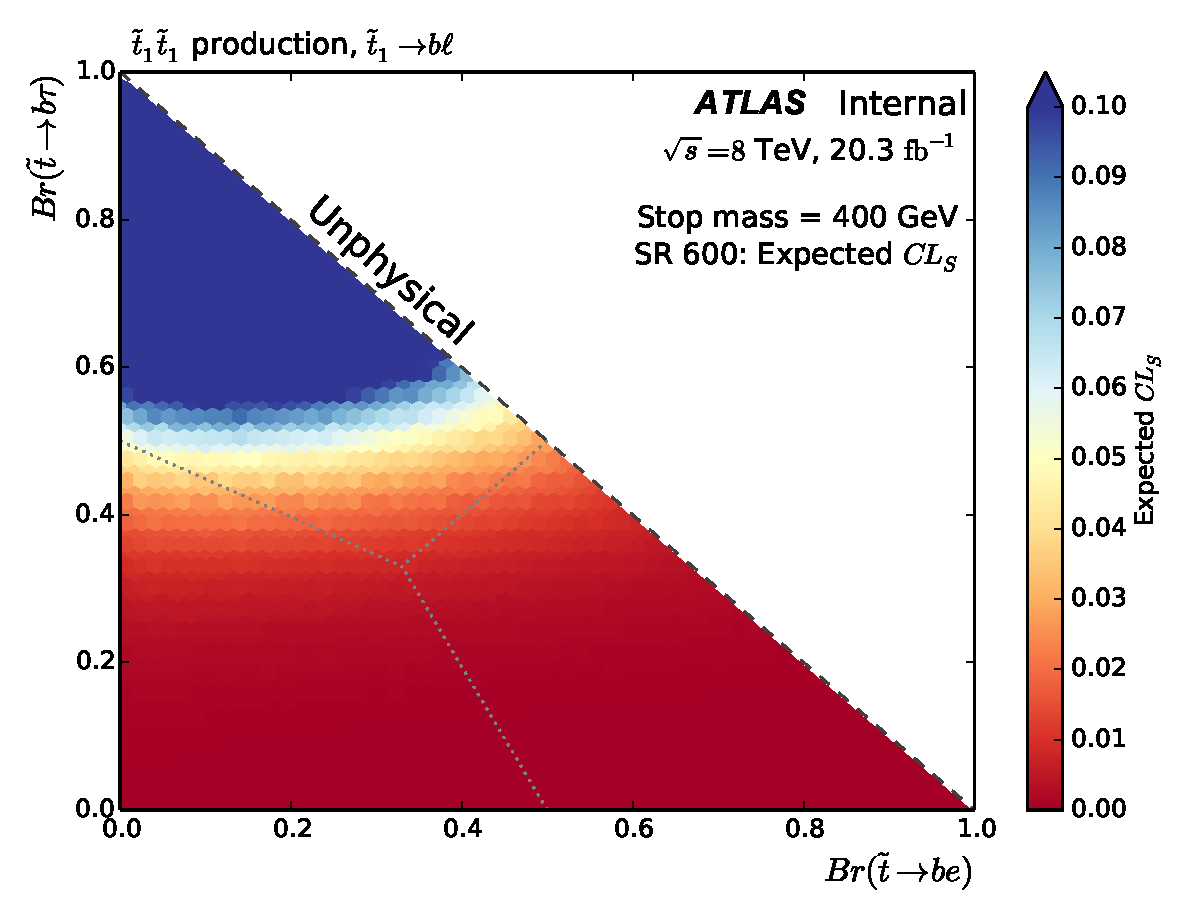
\includegraphics[width=0.65\textwidth]
      {figs/blstop/cls_plots/cls_vs_br_m_400_sr_600_exp.pdf}
  }
  \caption{
    Expected $CL_S$ values in SR~400 and SR~600 for a stop mass of 400~\GeV,
    shown across the plane of physical stop branching ratios.
  }
\end{figure}

\begin{figure}[ht]
  \centering
  \subbottom[Observed $CL_S$ or SR~400]{
    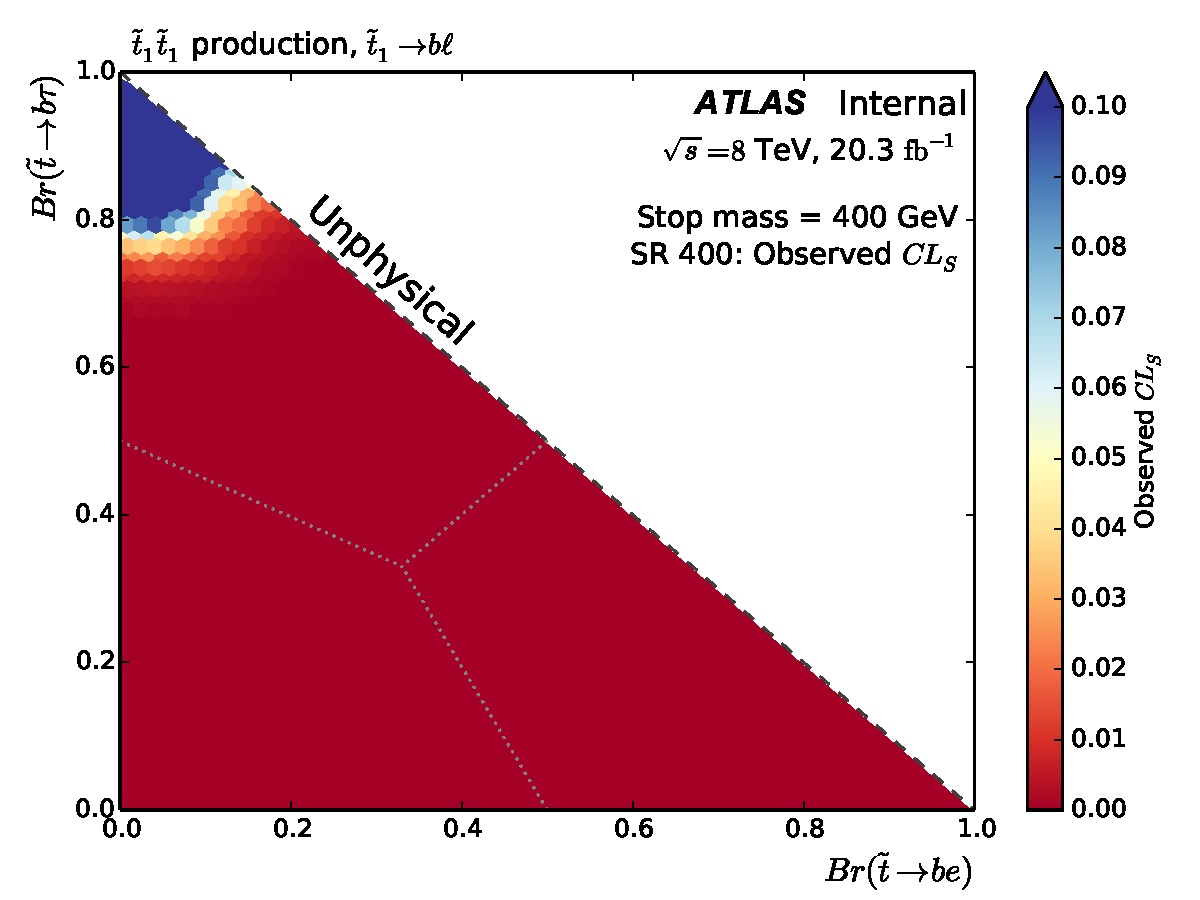
\includegraphics[width=0.65\textwidth]
      {figs/blstop/cls_plots/cls_vs_br_m_400_sr_400_obs.pdf}
  }
  \subbottom[Observed $CL_S$ or SR~600]{
    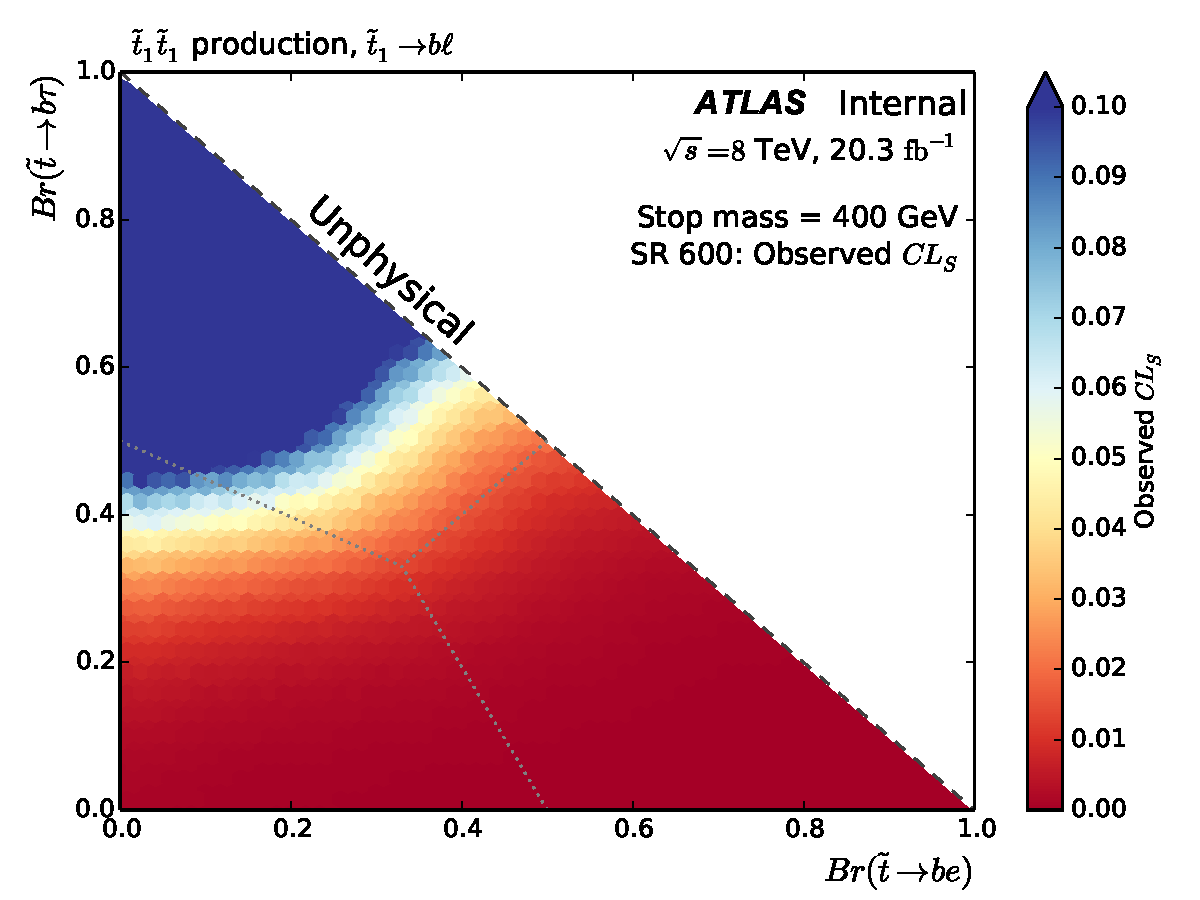
\includegraphics[width=0.65\textwidth]
      {figs/blstop/cls_plots/cls_vs_br_m_400_sr_600_obs.pdf}
  }
  \caption{
    Observed $CL_S$ values in SR~400 and SR~600 for a stop mass of 400~\GeV,
    shown across the plane of physical stop branching ratios.
  }
\end{figure}

\begin{figure}[ht]
  \centering
  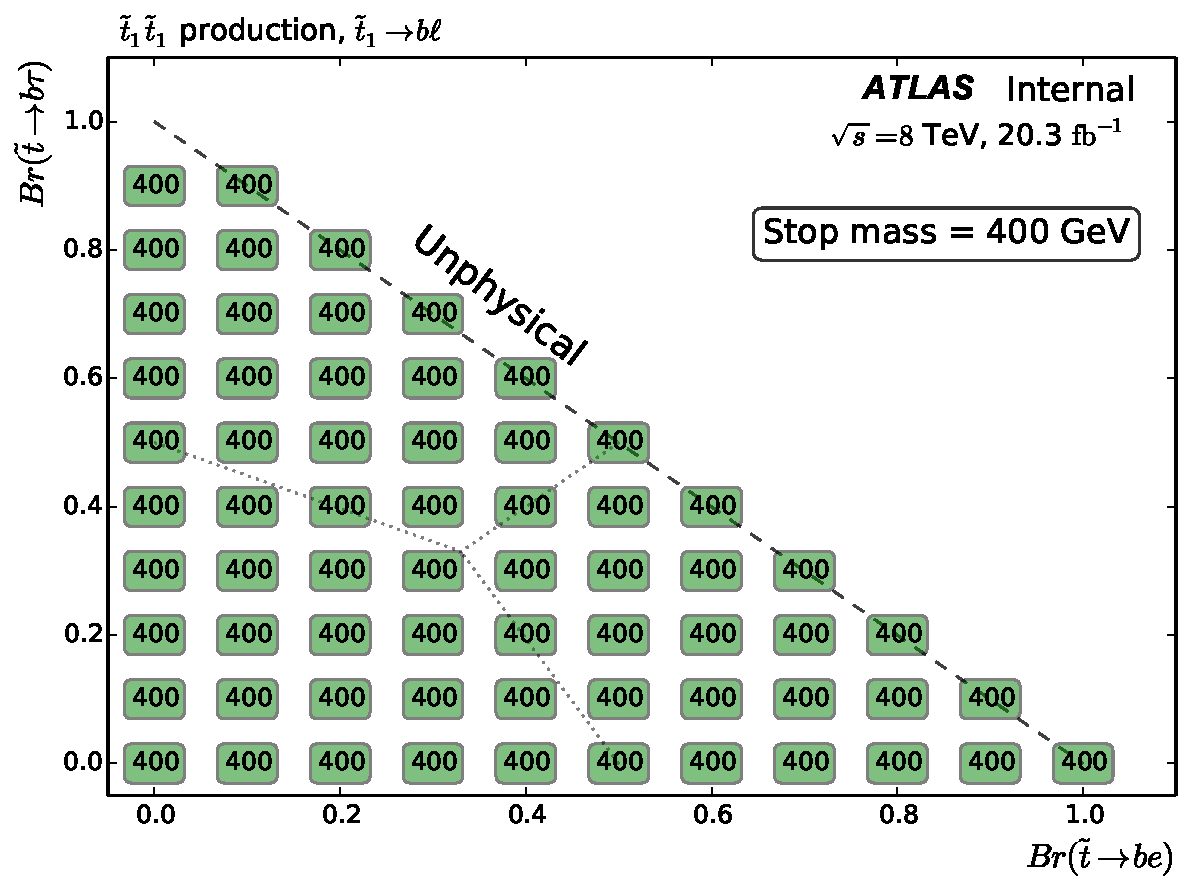
\includegraphics[width=0.65\textwidth]
    {figs/blstop/region_selection/region_choice_vs_br_m_400.pdf}
  \caption{
    Selected SR for select stop branching ratios for a stop mass of 400~\GeV.
    The SR is selected by choosing the SR with the smallest expected $CL_S$
    value for a given branching ratio.
    For several points in the branching ratio plane, SR~400 was selected because
    the two regions have the same expected $CL_S$ value, with the numerical
    precision of the statistical software.
    For these points, the expected sensitivity for both SRs is such that
    there is little difference between the expected sensitivity.
  }
\end{figure}

\FloatBarrier

%% -----------------------------------------------------------------------------
\newpage
\section{500 \texorpdfstring{\GeV}{GeV} stop mass}

\begin{figure}[ht]
  \centering
  \subbottom[Expected $CL_S$ or SR~400]{
    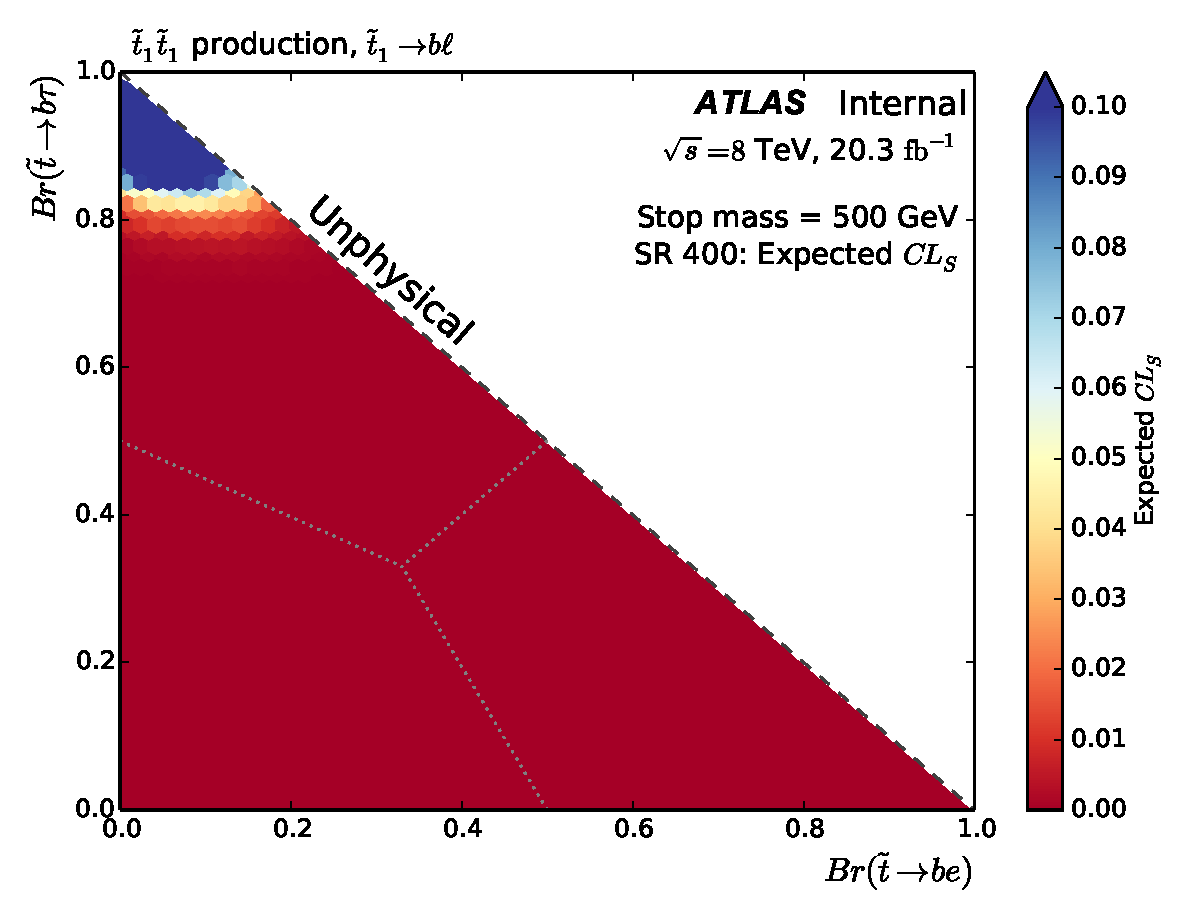
\includegraphics[width=0.65\textwidth]
      {figs/blstop/cls_plots/cls_vs_br_m_500_sr_400_exp.pdf}
  }
  \subbottom[Expected $CL_S$ or SR~600]{
    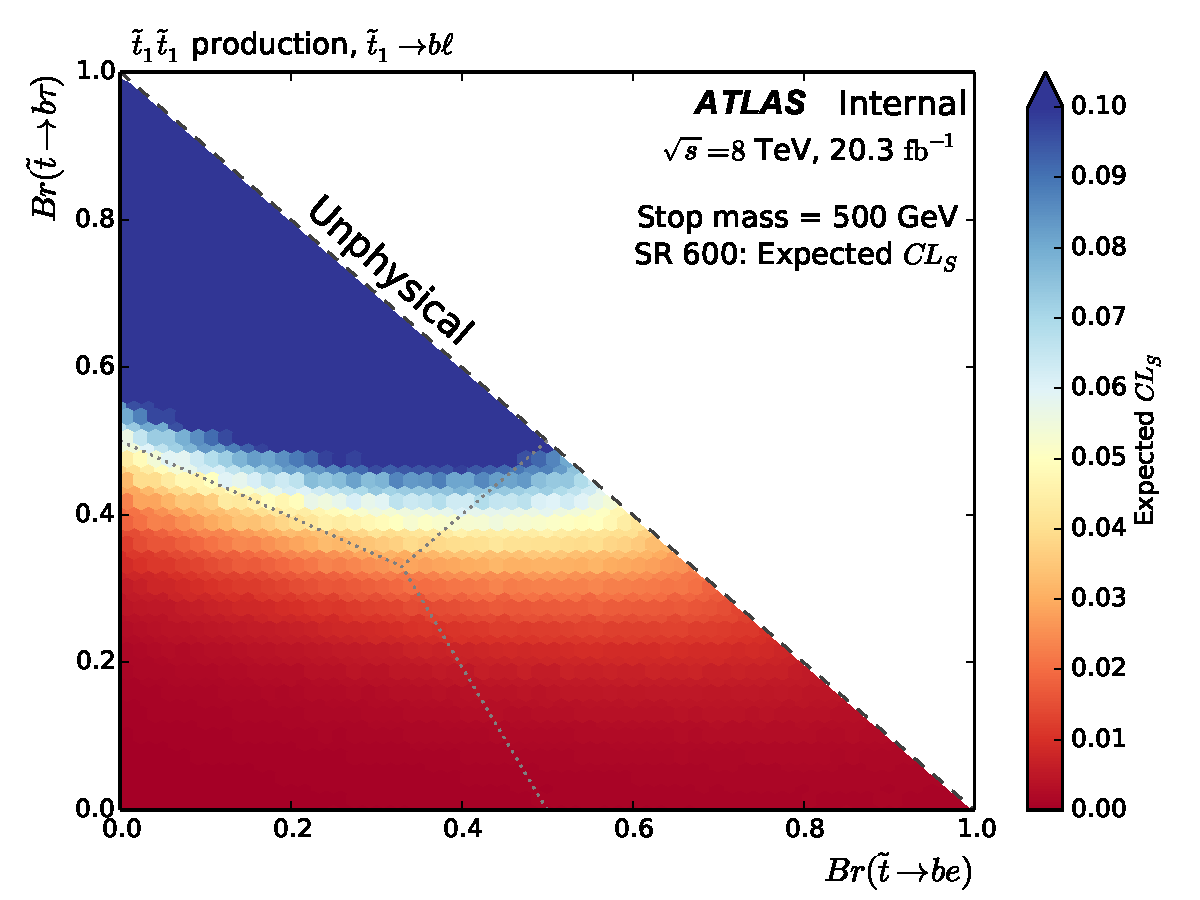
\includegraphics[width=0.65\textwidth]
      {figs/blstop/cls_plots/cls_vs_br_m_500_sr_600_exp.pdf}
  }
  \caption{
    Expected $CL_S$ values in SR~400 and SR~600 for a stop mass of 500~\GeV,
    shown across the plane of physical stop branching ratios.
  }
\end{figure}

\begin{figure}[ht]
  \centering
  \subbottom[Observed $CL_S$ or SR~400]{
    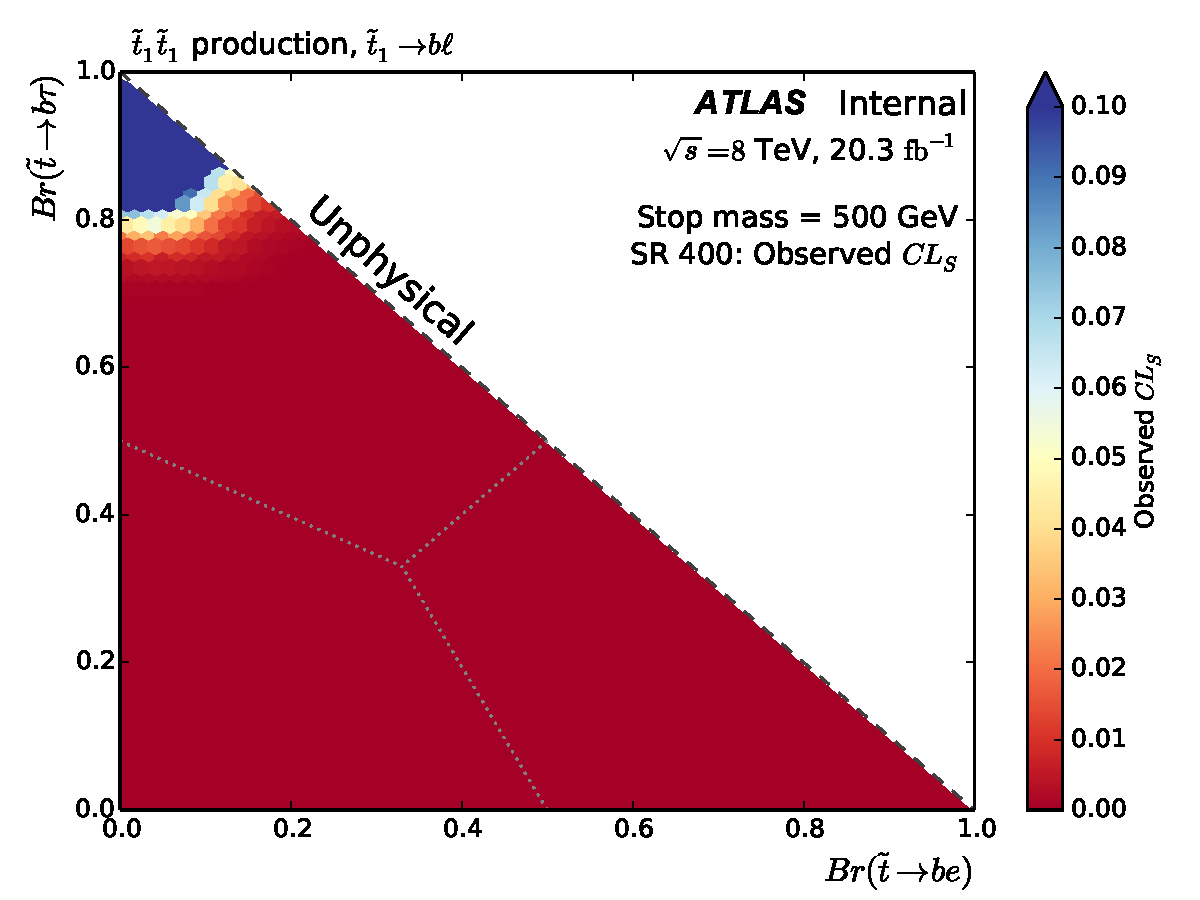
\includegraphics[width=0.65\textwidth]
      {figs/blstop/cls_plots/cls_vs_br_m_500_sr_400_obs.pdf}
  }
  \subbottom[Observed $CL_S$ or SR~600]{
    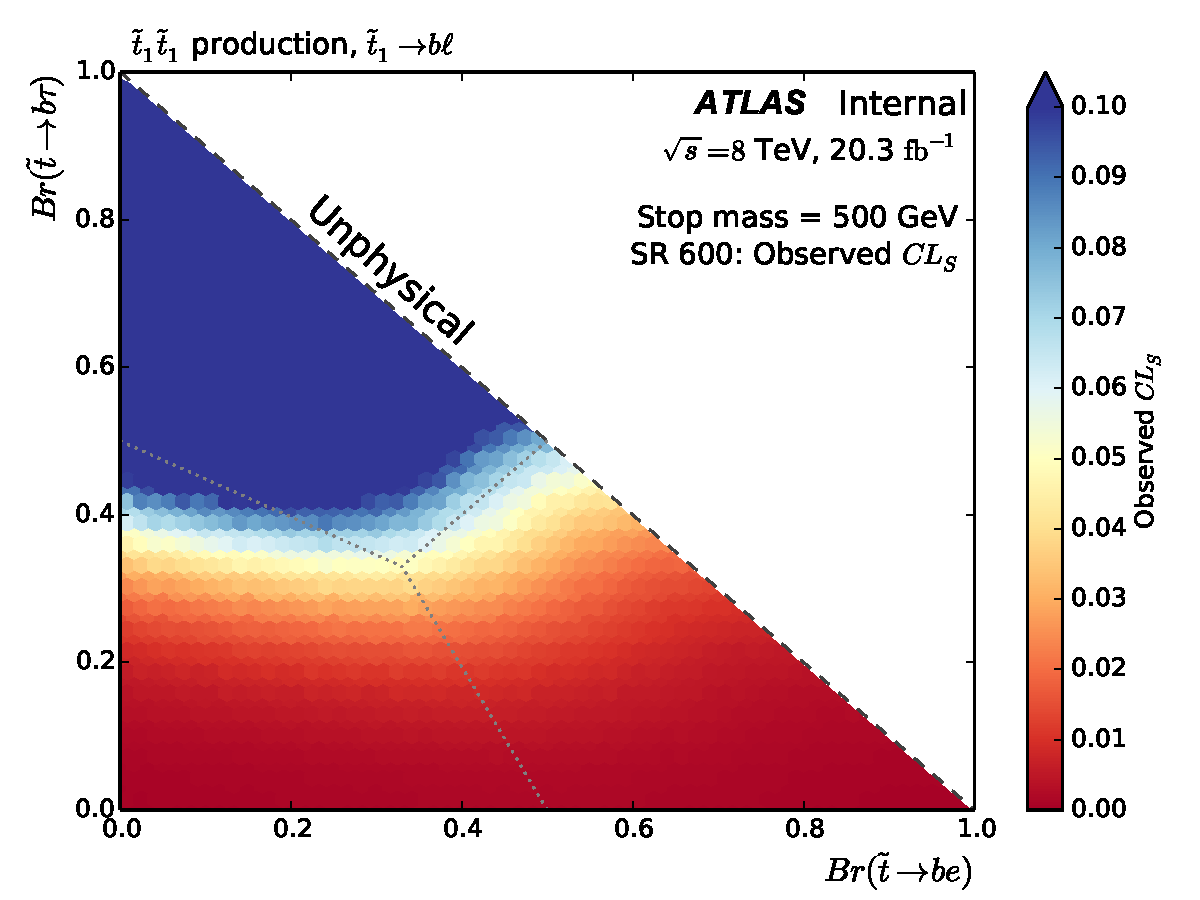
\includegraphics[width=0.65\textwidth]
      {figs/blstop/cls_plots/cls_vs_br_m_500_sr_600_obs.pdf}
  }
  \caption{
    Observed $CL_S$ values in SR~400 and SR~600 for a stop mass of 500~\GeV,
    shown across the plane of physical stop branching ratios.
  }
\end{figure}

\begin{figure}[ht]
  \centering
  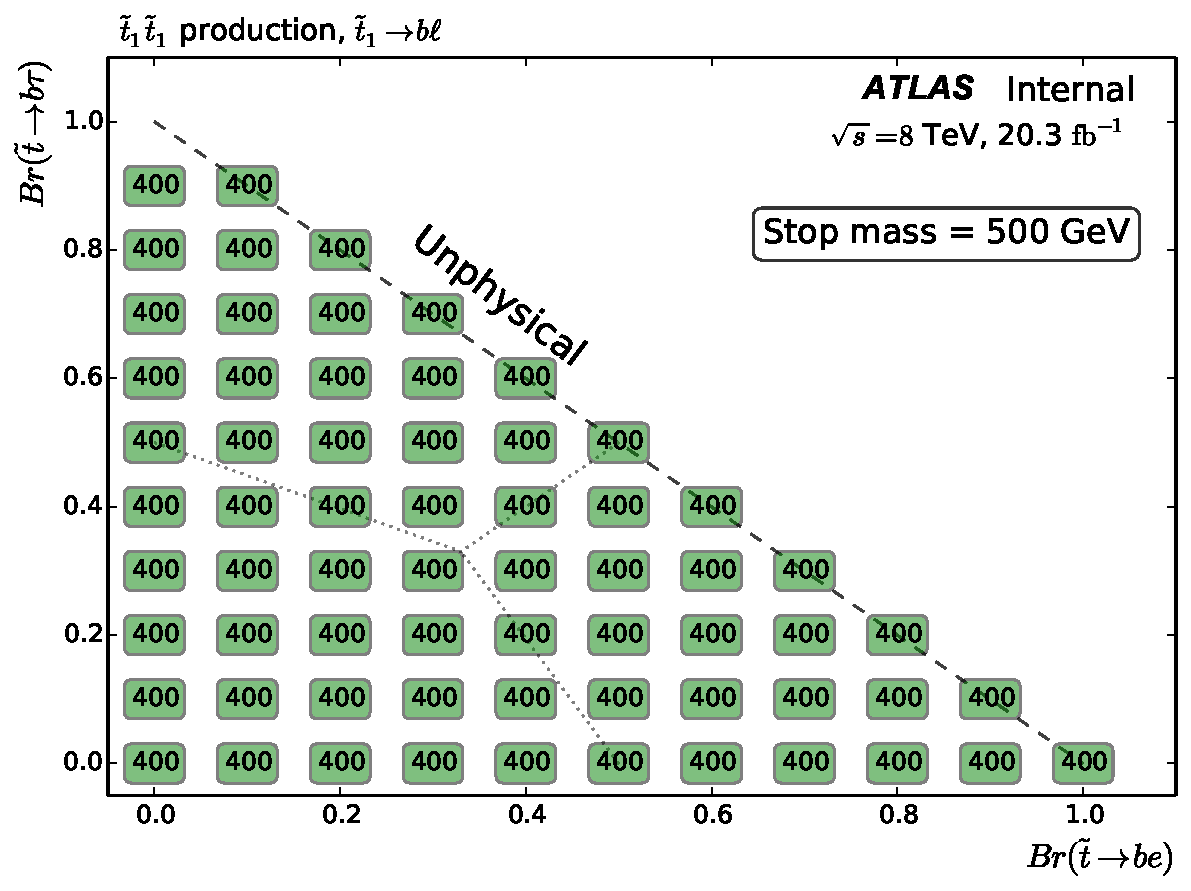
\includegraphics[width=0.65\textwidth]
    {figs/blstop/region_selection/region_choice_vs_br_m_500.pdf}
  \caption{
    Selected SR for select stop branching ratios for a stop mass of 500~\GeV.
    The SR is selected by choosing the SR with the smallest expected $CL_S$
    value for a given branching ratio.
    For several points in the branching ratio plane, SR~400 was selected because
    the two regions have the same expected $CL_S$ value, with the numerical
    precision of the statistical software.
    For these points, the expected sensitivity for both SRs is such that
    there is little difference between the expected sensitivity.
  }
\end{figure}

\FloatBarrier

%% -----------------------------------------------------------------------------
\newpage
\section{600 \texorpdfstring{\GeV}{GeV} stop mass}

\begin{figure}[ht]
  \centering
  \subbottom[Expected $CL_S$ or SR~400]{
    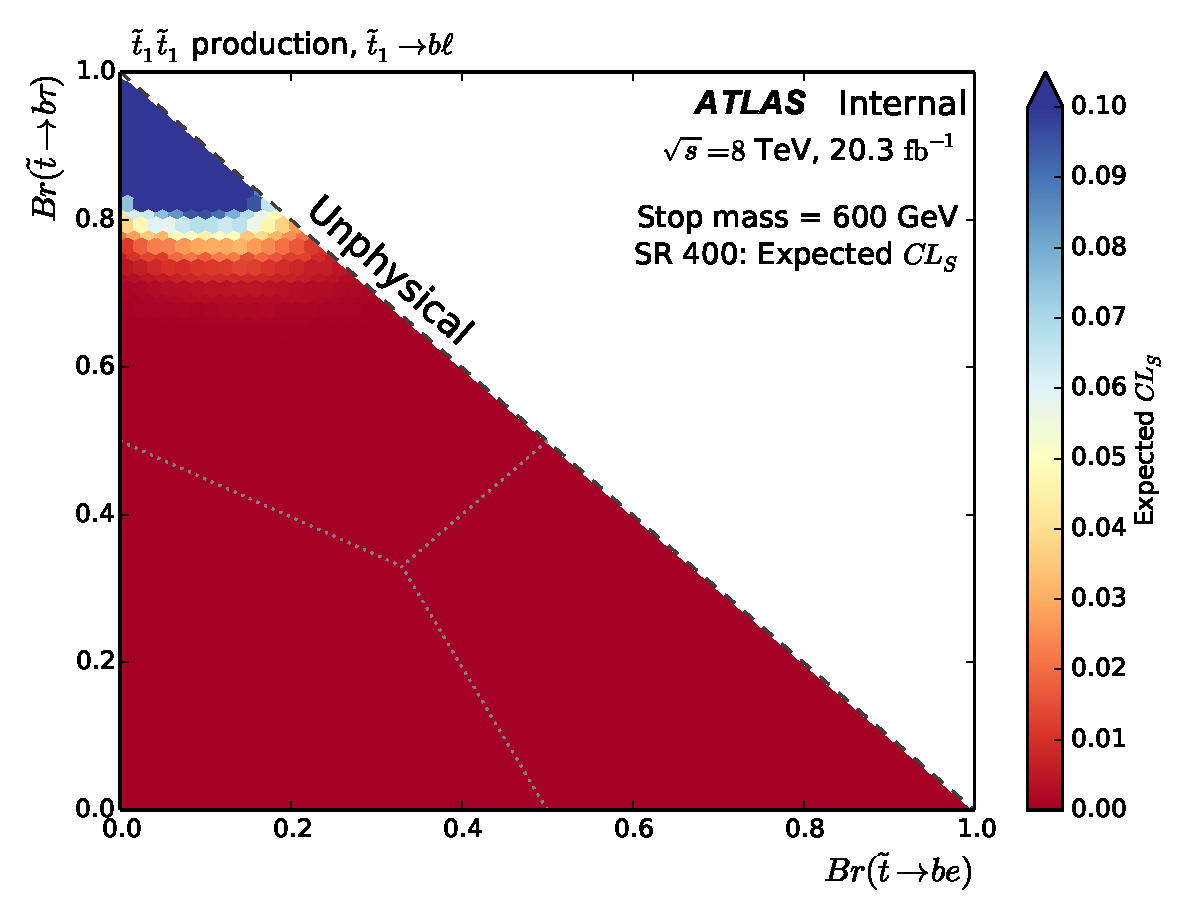
\includegraphics[width=0.65\textwidth]
      {figs/blstop/cls_plots/cls_vs_br_m_600_sr_400_exp.pdf}
  }
  \subbottom[Expected $CL_S$ or SR~600]{
    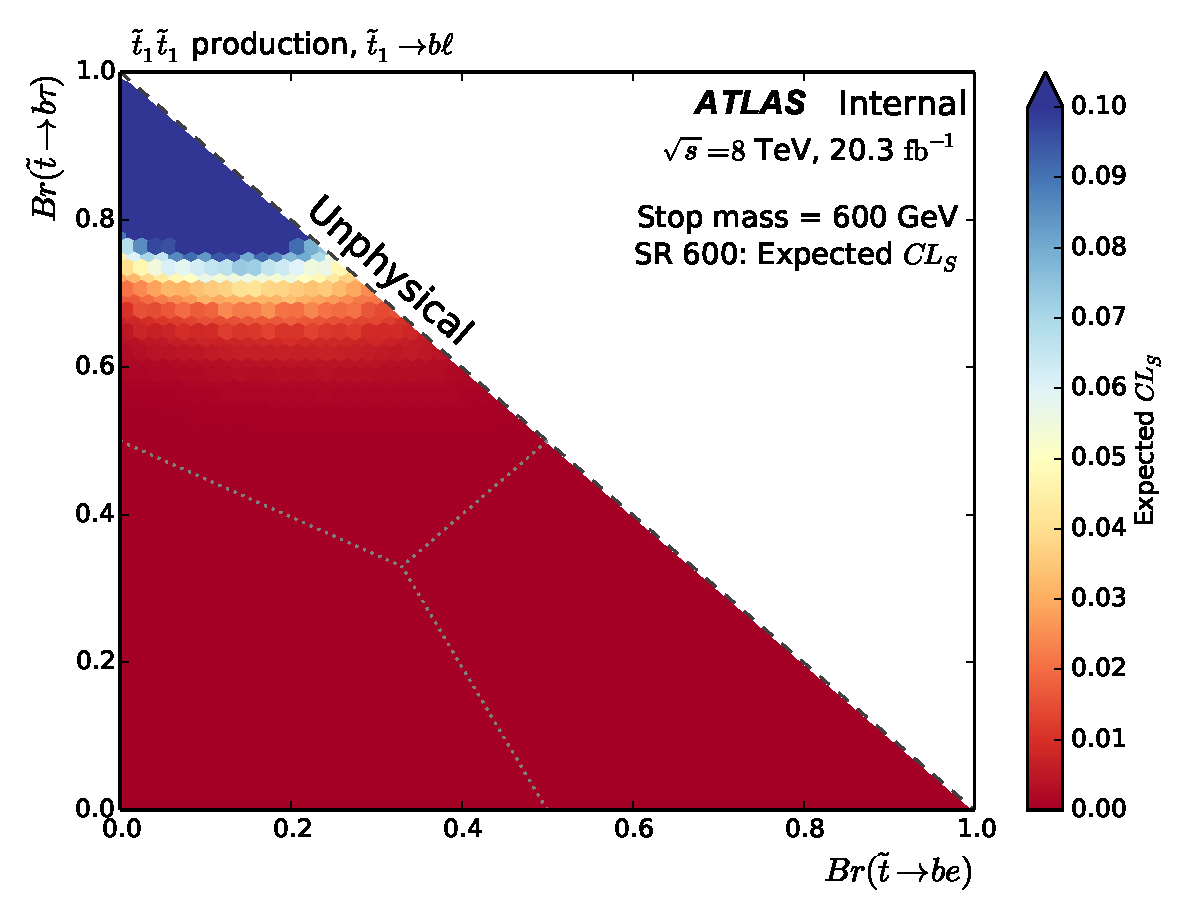
\includegraphics[width=0.65\textwidth]
      {figs/blstop/cls_plots/cls_vs_br_m_600_sr_600_exp.pdf}
  }
  \caption{
    Expected $CL_S$ values in SR~400 and SR~600 for a stop mass of 600~\GeV,
    shown across the plane of physical stop branching ratios.
  }
\end{figure}

\begin{figure}[ht]
  \centering
  \subbottom[Observed $CL_S$ or SR~400]{
    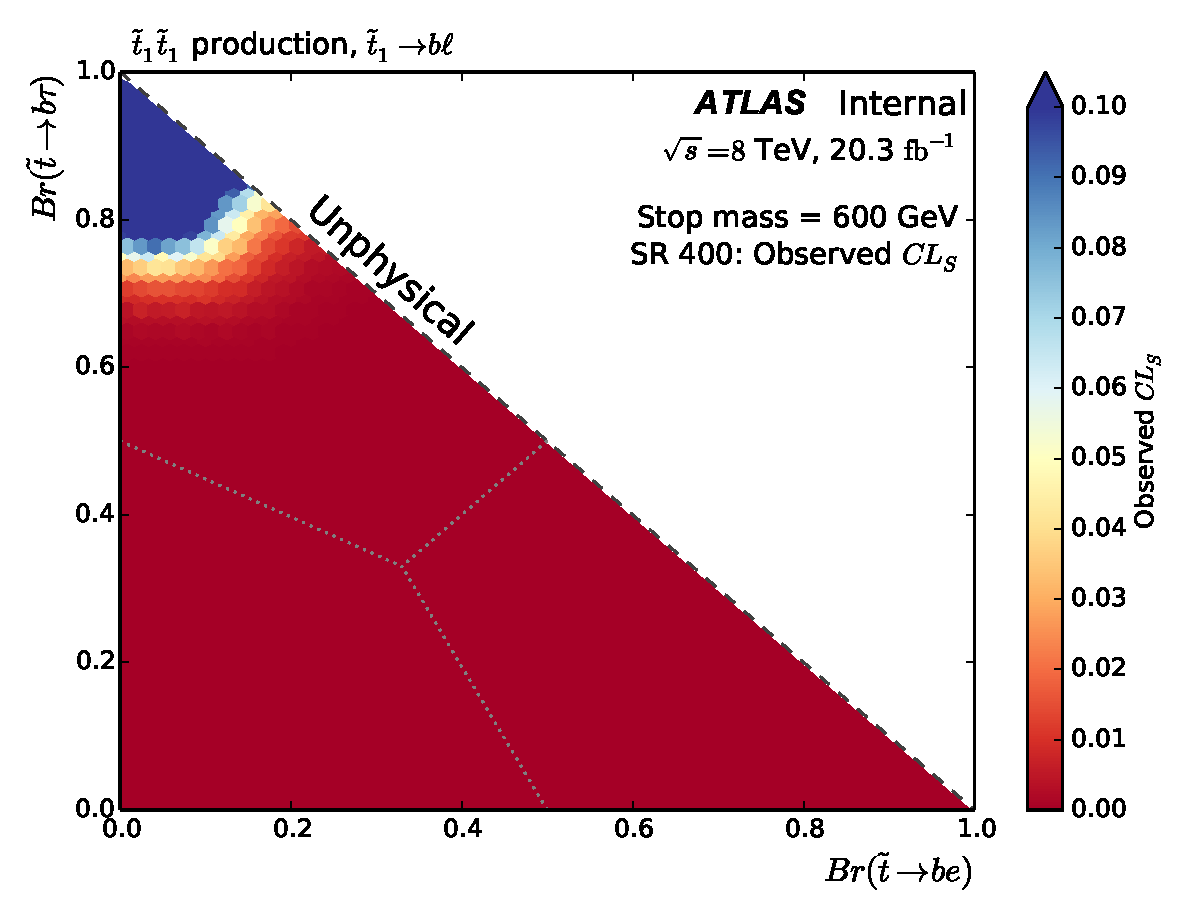
\includegraphics[width=0.65\textwidth]
      {figs/blstop/cls_plots/cls_vs_br_m_600_sr_400_obs.pdf}
  }
  \subbottom[Observed $CL_S$ or SR~600]{
    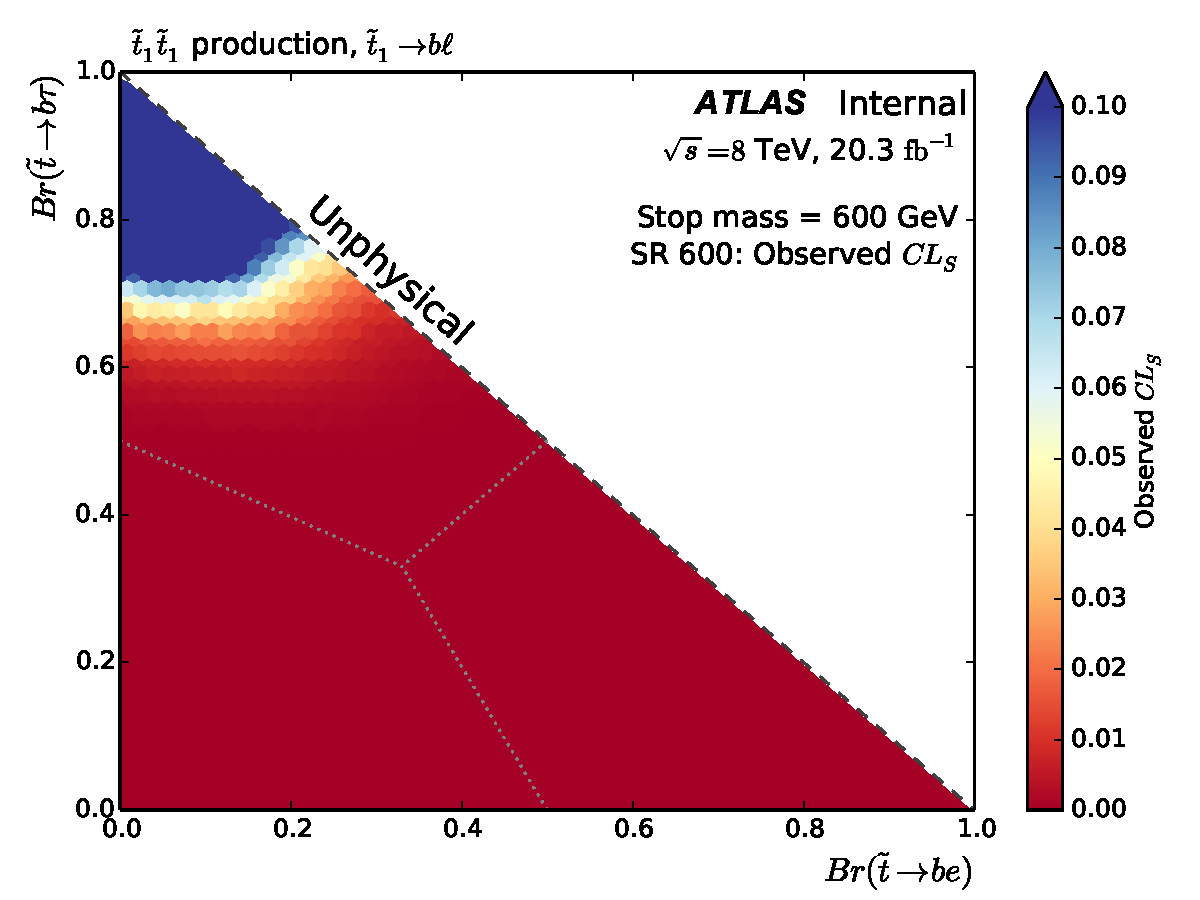
\includegraphics[width=0.65\textwidth]
      {figs/blstop/cls_plots/cls_vs_br_m_600_sr_600_obs.pdf}
  }
  \caption{
    Observed $CL_S$ values in SR~400 and SR~600 for a stop mass of 600~\GeV,
    shown across the plane of physical stop branching ratios.
  }
\end{figure}

\begin{figure}[ht]
  \centering
  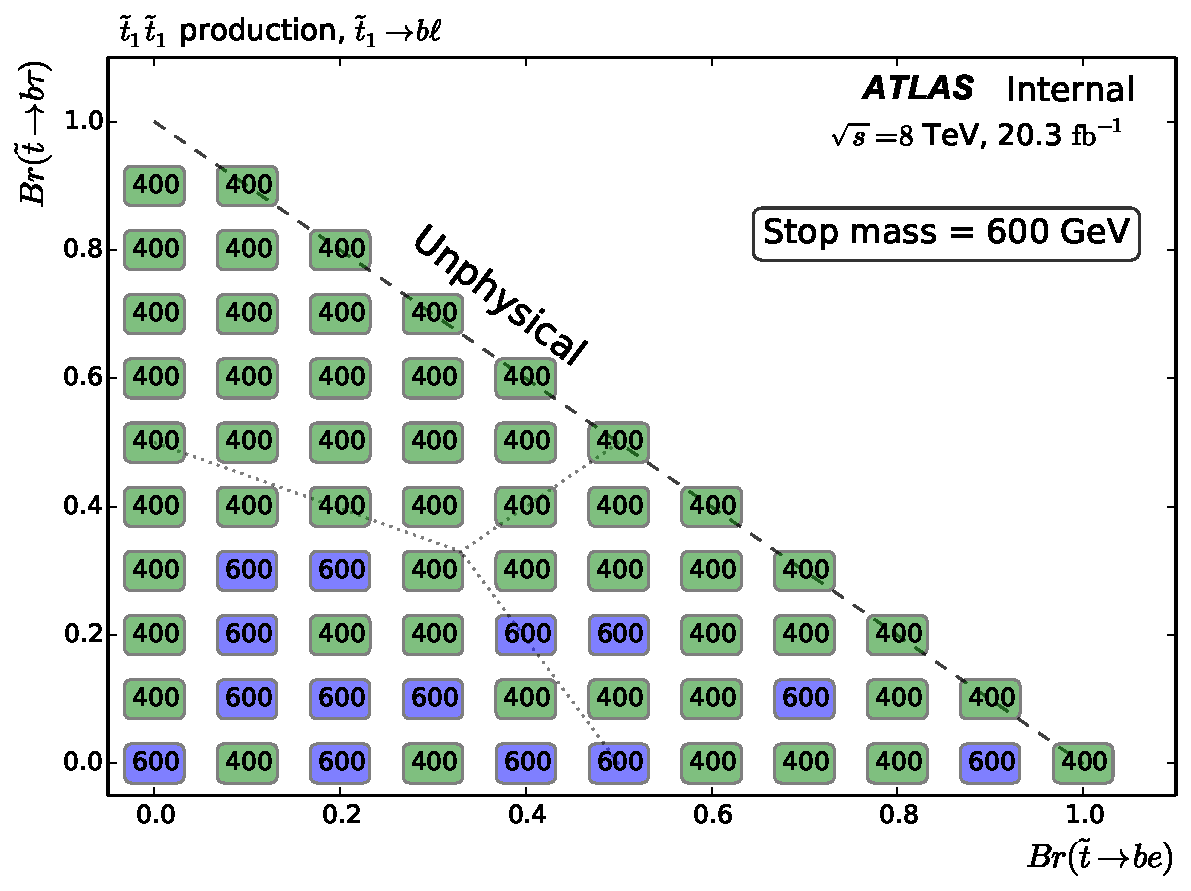
\includegraphics[width=0.65\textwidth]
    {figs/blstop/region_selection/region_choice_vs_br_m_600.pdf}
  \caption{
    Selected SR for select stop branching ratios for a stop mass of 600~\GeV.
    The SR is selected by choosing the SR with the smallest expected $CL_S$
    value for a given branching ratio.
    For several points in the branching ratio plane, SR~400 was selected because
    the two regions have the same expected $CL_S$ value, with the numerical
    precision of the statistical software.
    For these points, the expected sensitivity for both SRs is such that
    there is little difference between the expected sensitivity.
  }
\end{figure}

\FloatBarrier

%% -----------------------------------------------------------------------------
\newpage
\section{700 \texorpdfstring{\GeV}{GeV} stop mass}

\begin{figure}[ht]
  \centering
  \subbottom[Expected $CL_S$ or SR~400]{
    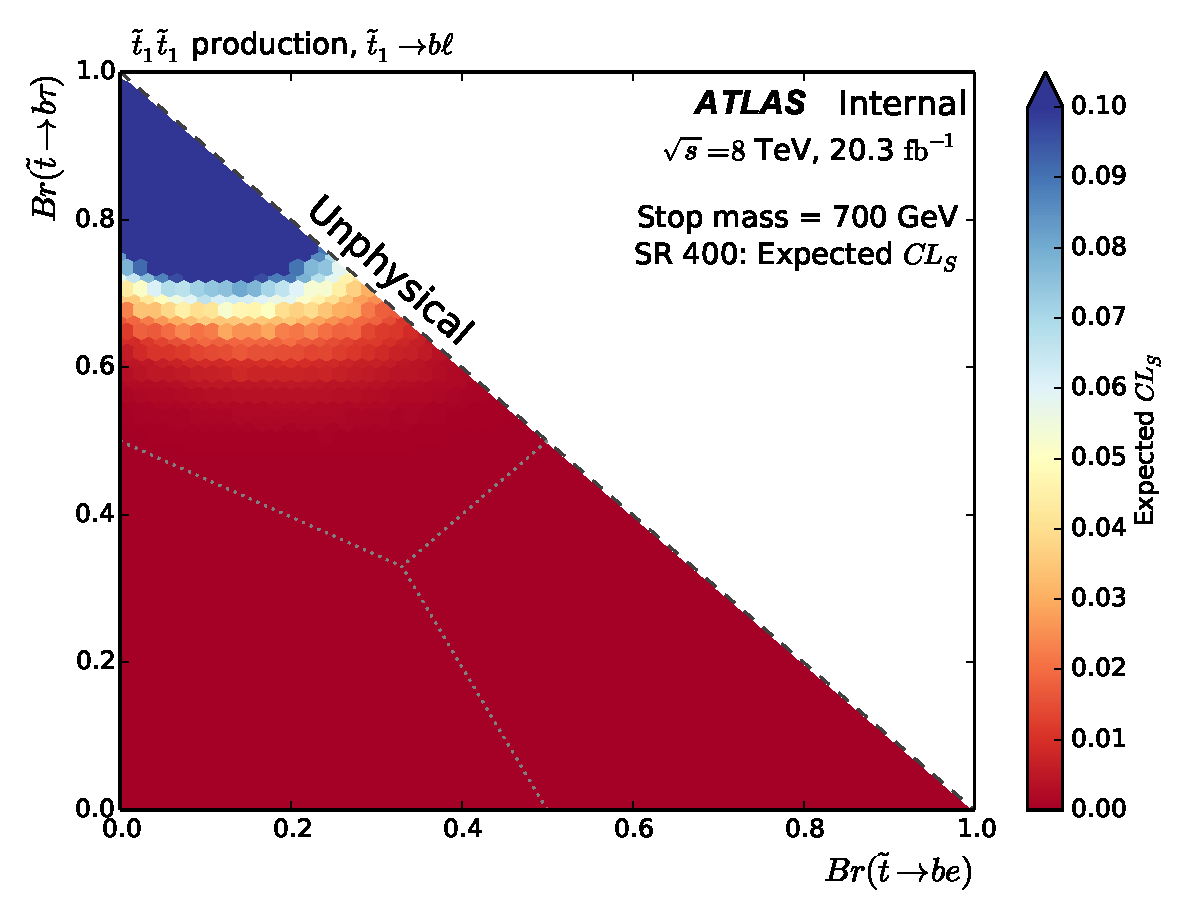
\includegraphics[width=0.65\textwidth]
      {figs/blstop/cls_plots/cls_vs_br_m_700_sr_400_exp.pdf}
  }
  \subbottom[Expected $CL_S$ or SR~600]{
    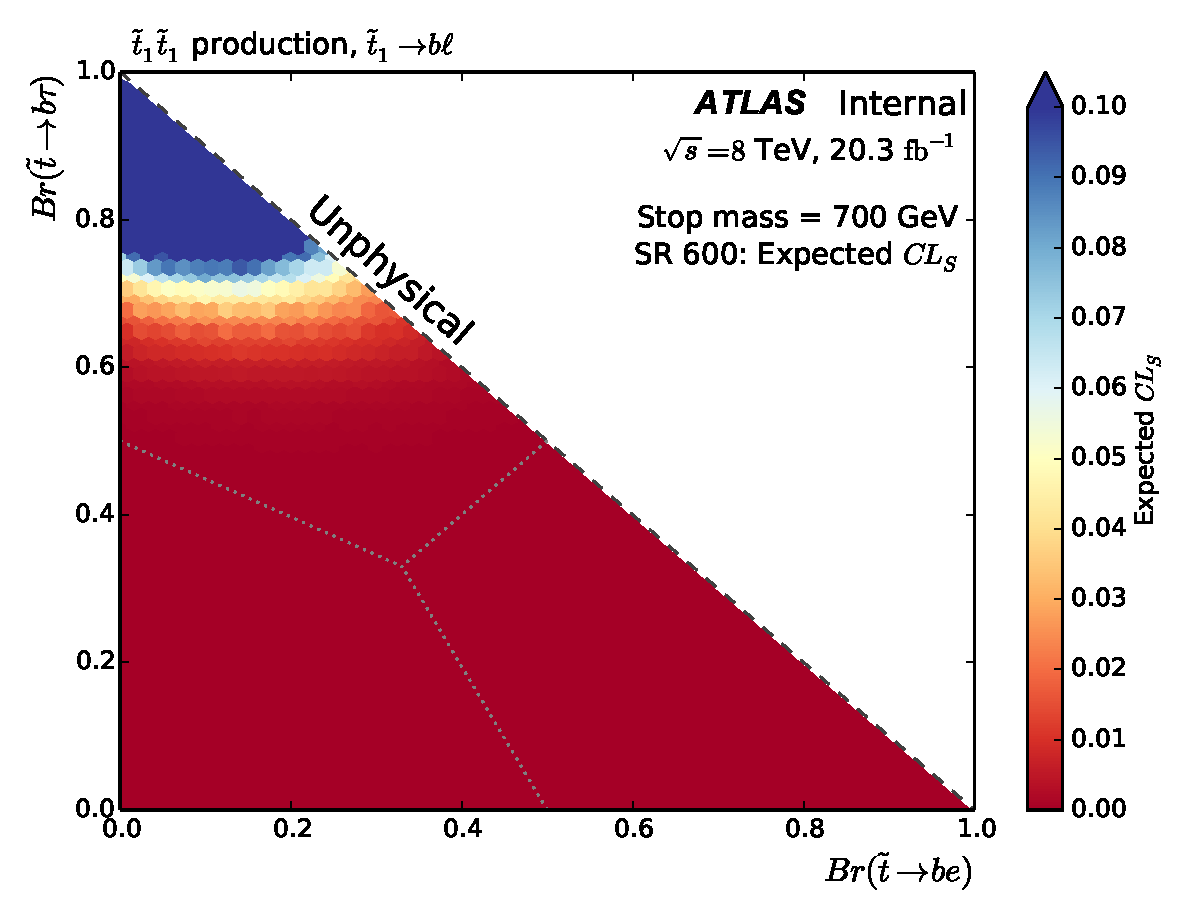
\includegraphics[width=0.65\textwidth]
      {figs/blstop/cls_plots/cls_vs_br_m_700_sr_600_exp.pdf}
  }
  \caption{
    Expected $CL_S$ values in SR~400 and SR~600 for a stop mass of 700~\GeV,
    shown across the plane of physical stop branching ratios.
  }
\end{figure}

\begin{figure}[ht]
  \centering
  \subbottom[Observed $CL_S$ or SR~400]{
    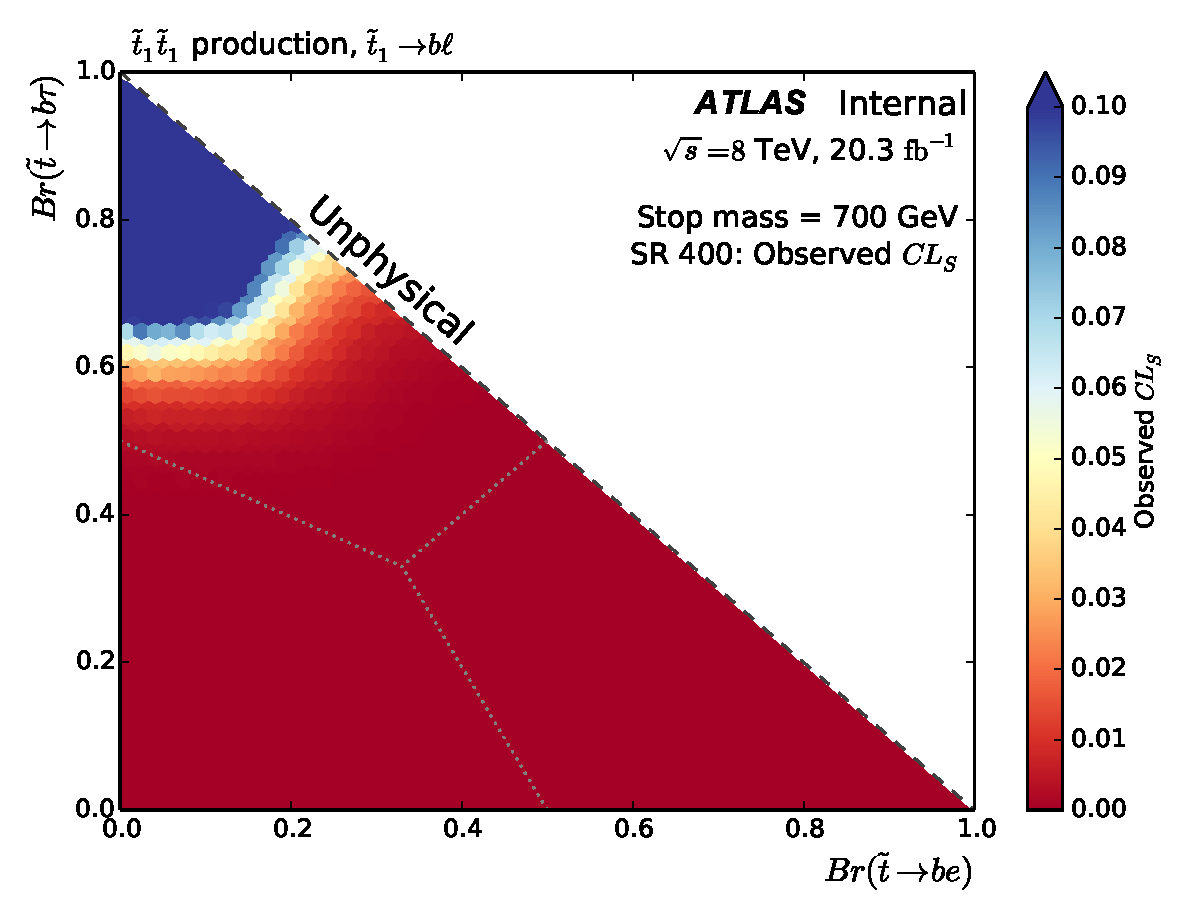
\includegraphics[width=0.65\textwidth]
      {figs/blstop/cls_plots/cls_vs_br_m_700_sr_400_obs.pdf}
  }
  \subbottom[Observed $CL_S$ or SR~600]{
    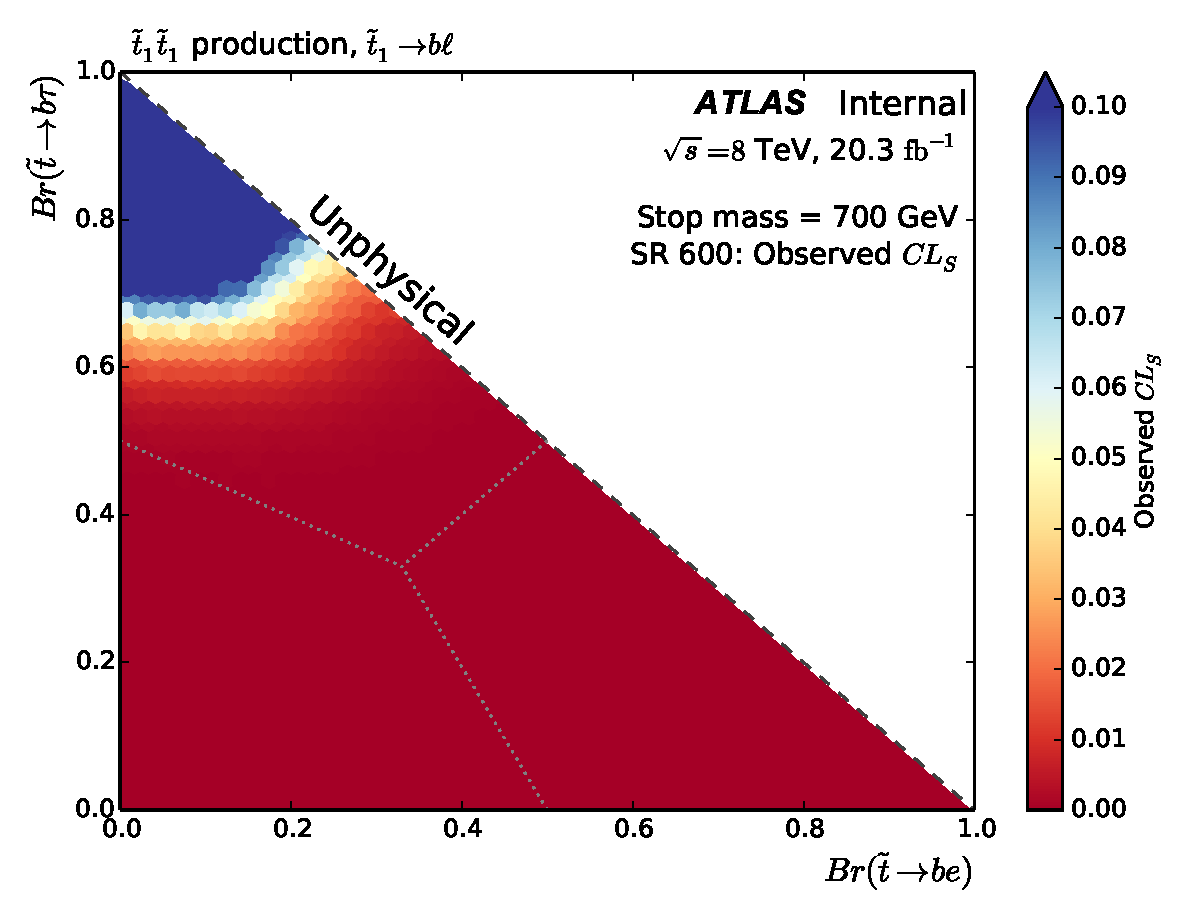
\includegraphics[width=0.65\textwidth]
      {figs/blstop/cls_plots/cls_vs_br_m_700_sr_600_obs.pdf}
  }
  \caption{
    Observed $CL_S$ values in SR~400 and SR~600 for a stop mass of 700~\GeV,
    shown across the plane of physical stop branching ratios.
  }
\end{figure}

\begin{figure}[ht]
  \centering
  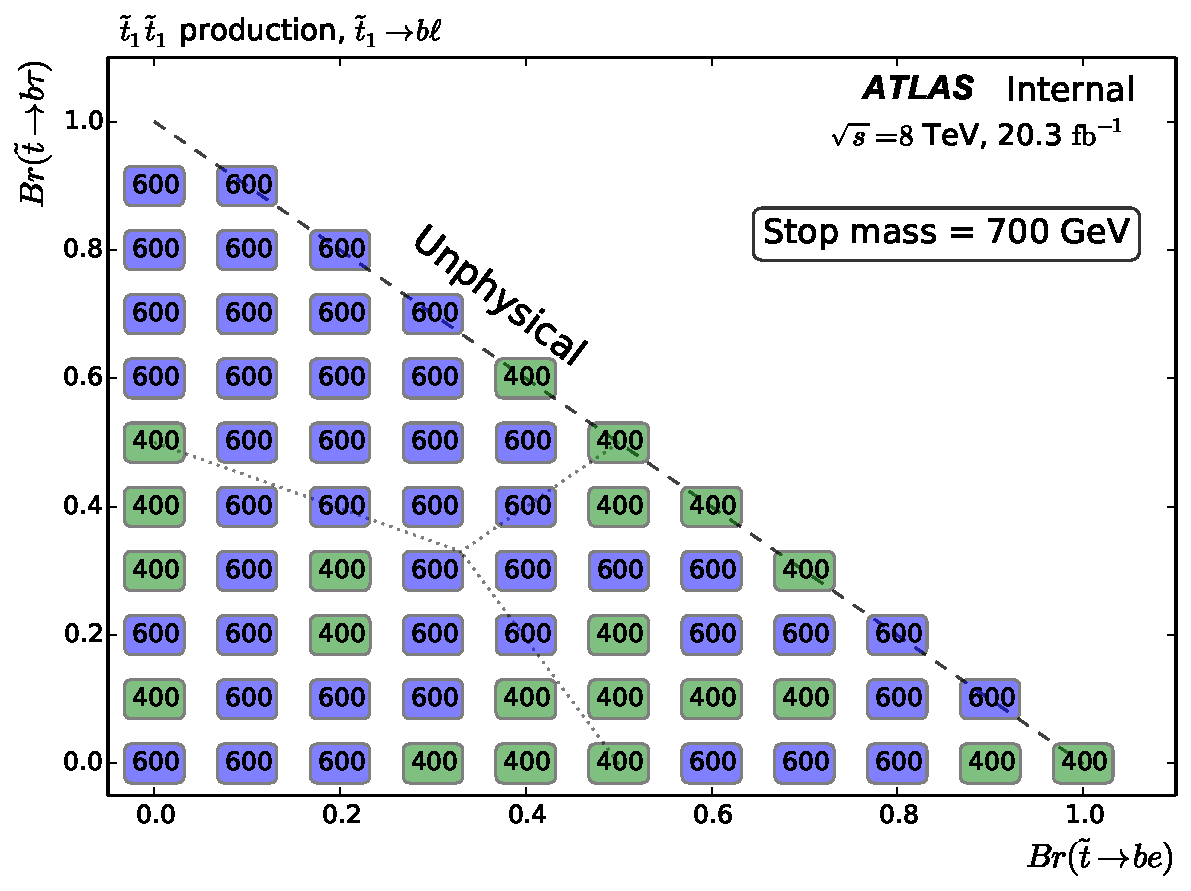
\includegraphics[width=0.65\textwidth]
    {figs/blstop/region_selection/region_choice_vs_br_m_700.pdf}
  \caption{
    Selected SR for select stop branching ratios for a stop mass of 700~\GeV.
    The SR is selected by choosing the SR with the smallest expected $CL_S$
    value for a given branching ratio.
    For several points in the branching ratio plane, SR~400 was selected because
    the two regions have the same expected $CL_S$ value, with the numerical
    precision of the statistical software.
    For these points, the expected sensitivity for both SRs is such that
    there is little difference between the expected sensitivity.
  }
\end{figure}

\FloatBarrier

%% -----------------------------------------------------------------------------
\newpage
\section{800 \texorpdfstring{\GeV}{GeV} stop mass}

\begin{figure}[ht]
  \centering
  \subbottom[Expected $CL_S$ or SR~400]{
    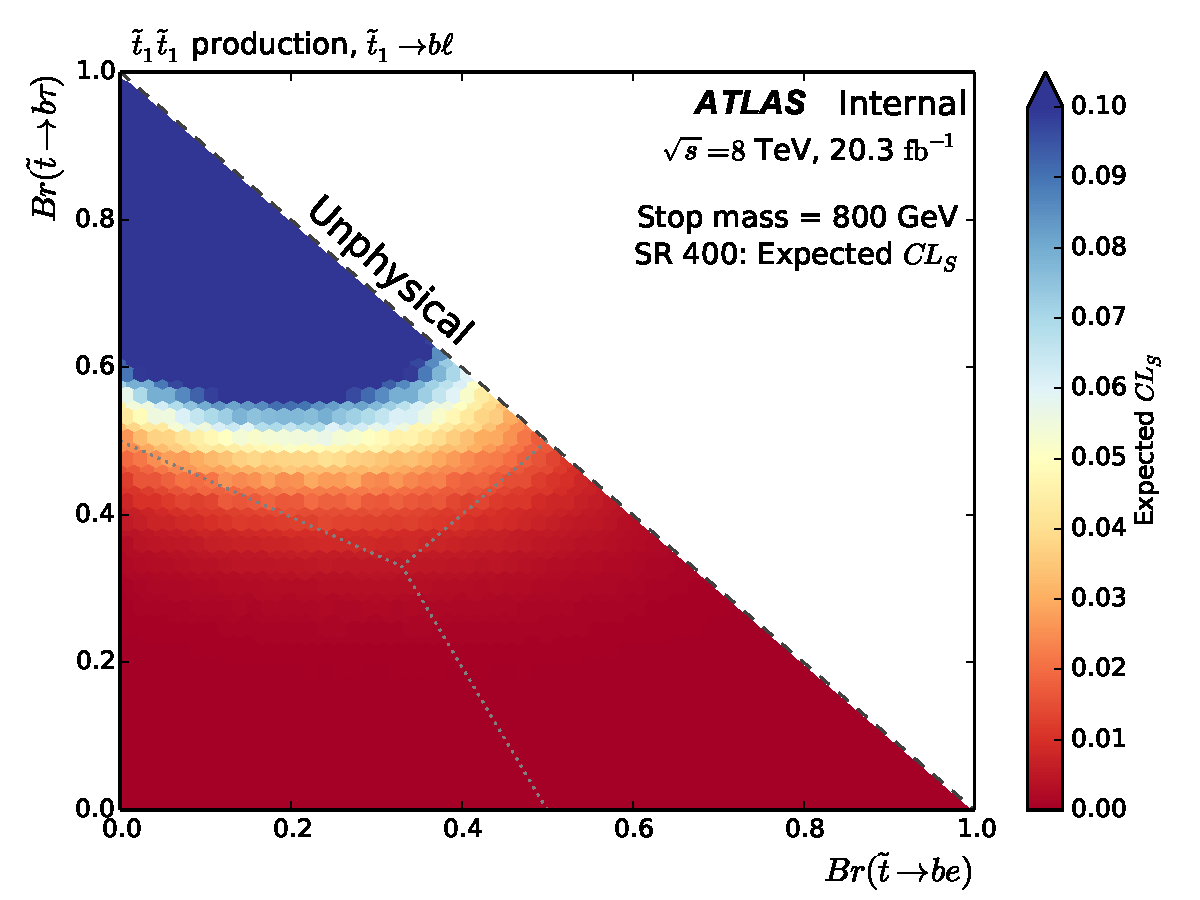
\includegraphics[width=0.65\textwidth]
      {figs/blstop/cls_plots/cls_vs_br_m_800_sr_400_exp.pdf}
  }
  \subbottom[Expected $CL_S$ or SR~600]{
    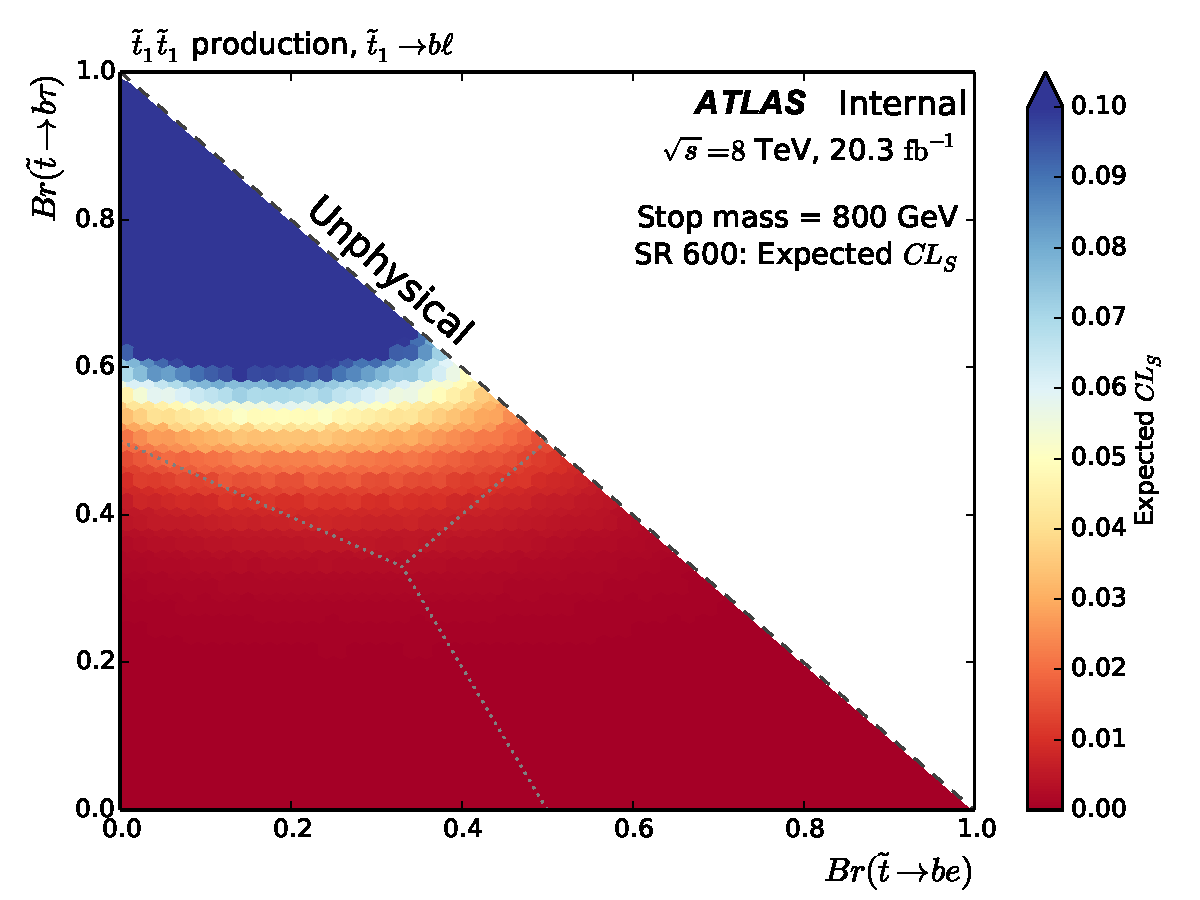
\includegraphics[width=0.65\textwidth]
      {figs/blstop/cls_plots/cls_vs_br_m_800_sr_600_exp.pdf}
  }
  \caption{
    Expected $CL_S$ values in SR~400 and SR~600 for a stop mass of 800~\GeV,
    shown across the plane of physical stop branching ratios.
  }
\end{figure}

\begin{figure}[ht]
  \centering
  \subbottom[Observed $CL_S$ or SR~400]{
    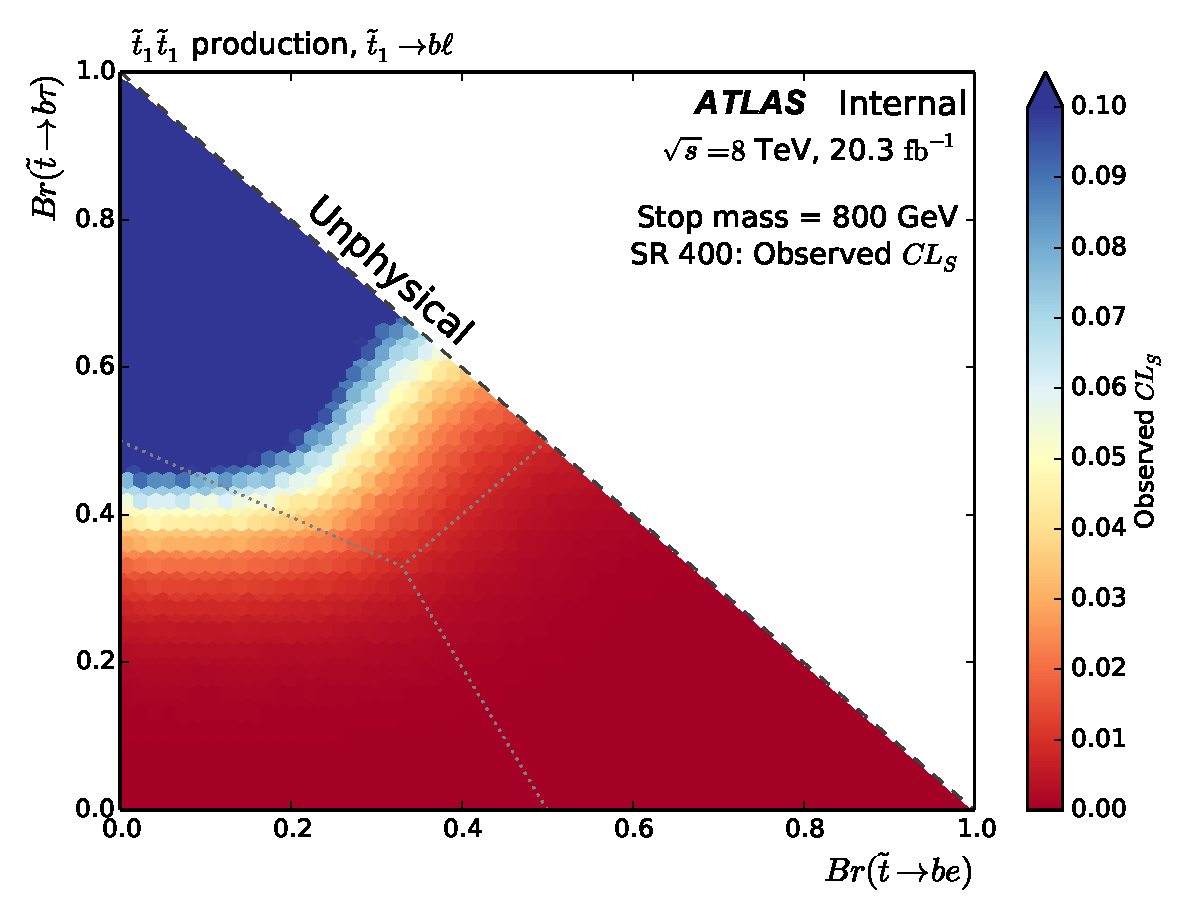
\includegraphics[width=0.65\textwidth]
      {figs/blstop/cls_plots/cls_vs_br_m_800_sr_400_obs.pdf}
  }
  \subbottom[Observed $CL_S$ or SR~600]{
    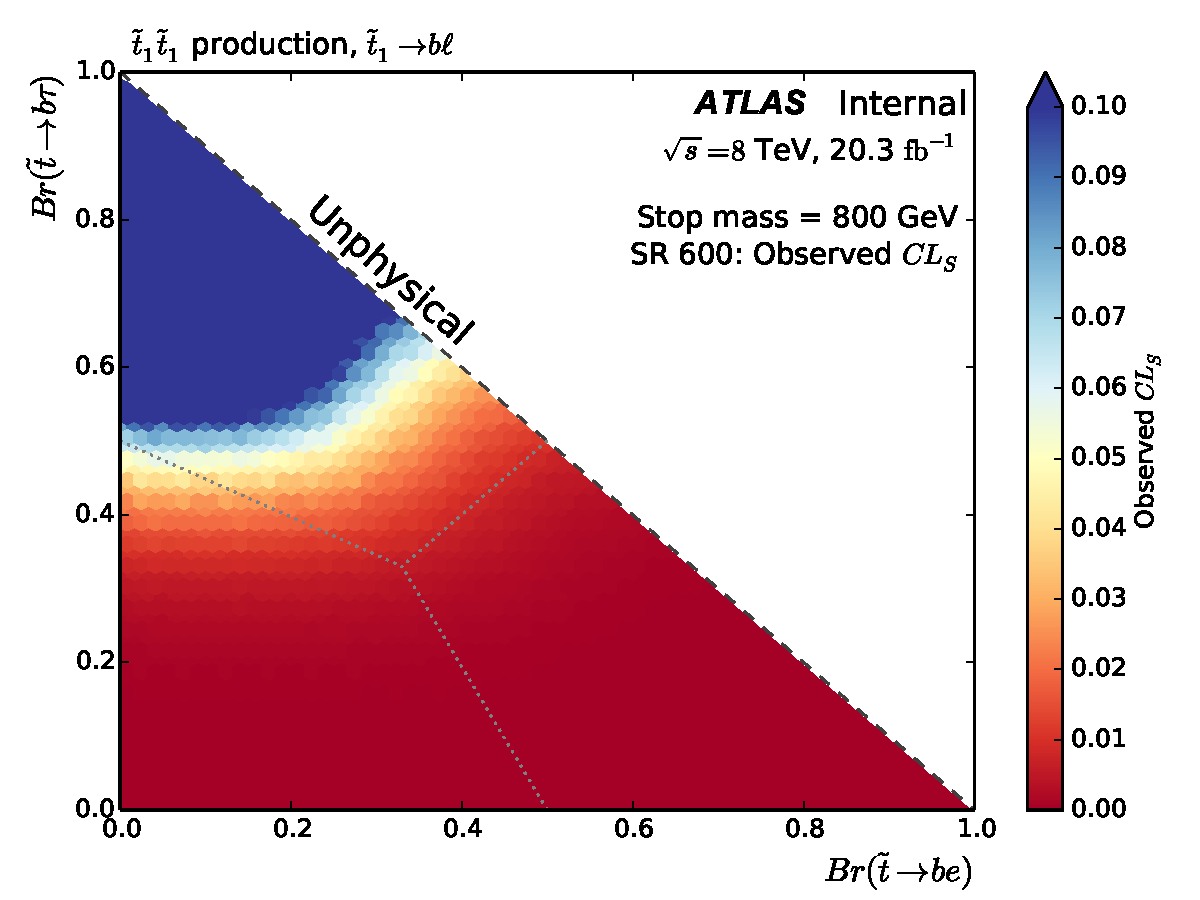
\includegraphics[width=0.65\textwidth]
      {figs/blstop/cls_plots/cls_vs_br_m_800_sr_600_obs.pdf}
  }
  \caption{
    Observed $CL_S$ values in SR~400 and SR~600 for a stop mass of 800~\GeV,
    shown across the plane of physical stop branching ratios.
  }
\end{figure}

\begin{figure}[ht]
  \centering
  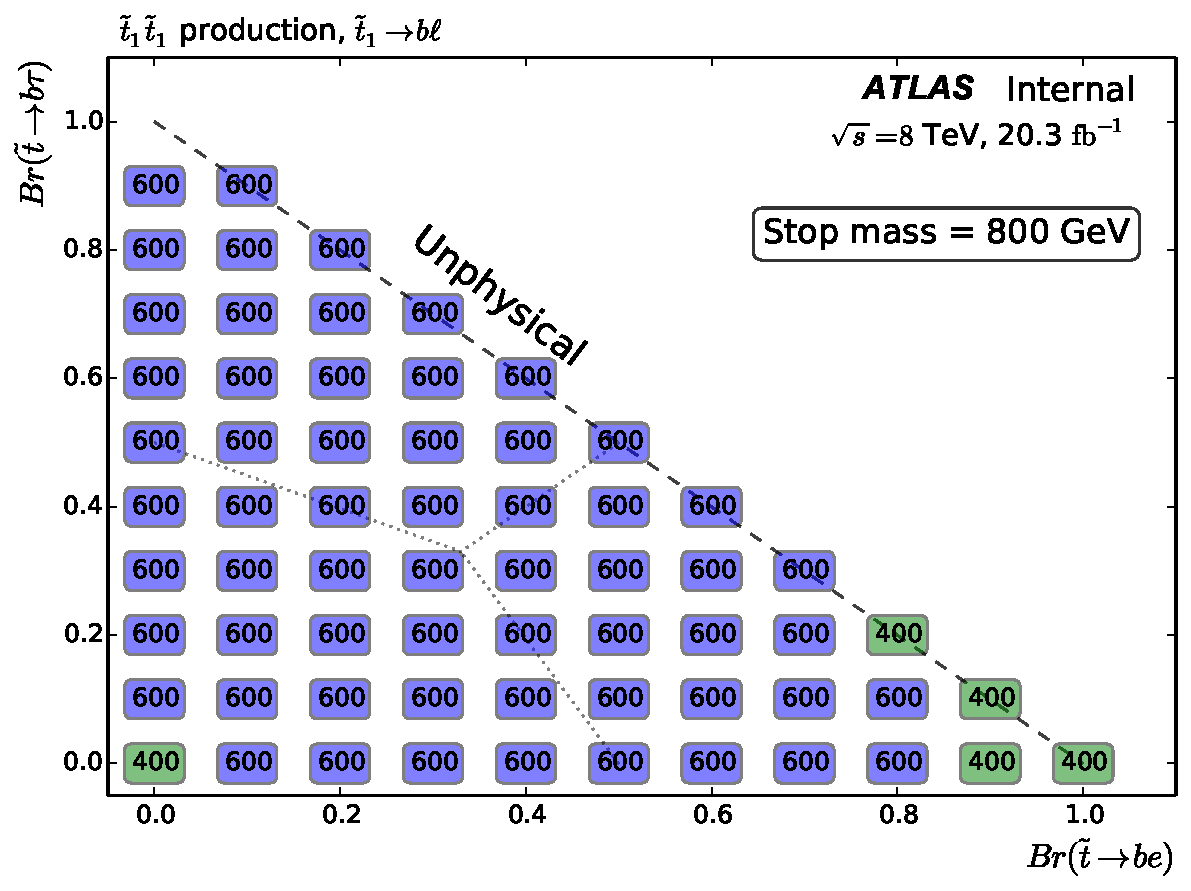
\includegraphics[width=0.65\textwidth]
    {figs/blstop/region_selection/region_choice_vs_br_m_800.pdf}
  \caption{
    Selected SR for select stop branching ratios for a stop mass of 800~\GeV.
    The SR is selected by choosing the SR with the smallest expected $CL_S$
    value for a given branching ratio.
    For several points in the branching ratio plane, SR~400 was selected because
    the two regions have the same expected $CL_S$ value, with the numerical
    precision of the statistical software.
    For these points, the expected sensitivity for both SRs is such that
    there is little difference between the expected sensitivity.
  }
\end{figure}

\FloatBarrier

%% -----------------------------------------------------------------------------
\newpage
\section{900 \texorpdfstring{\GeV}{GeV} stop mass}

\begin{figure}[ht]
  \centering
  \subbottom[Expected $CL_S$ or SR~400]{
    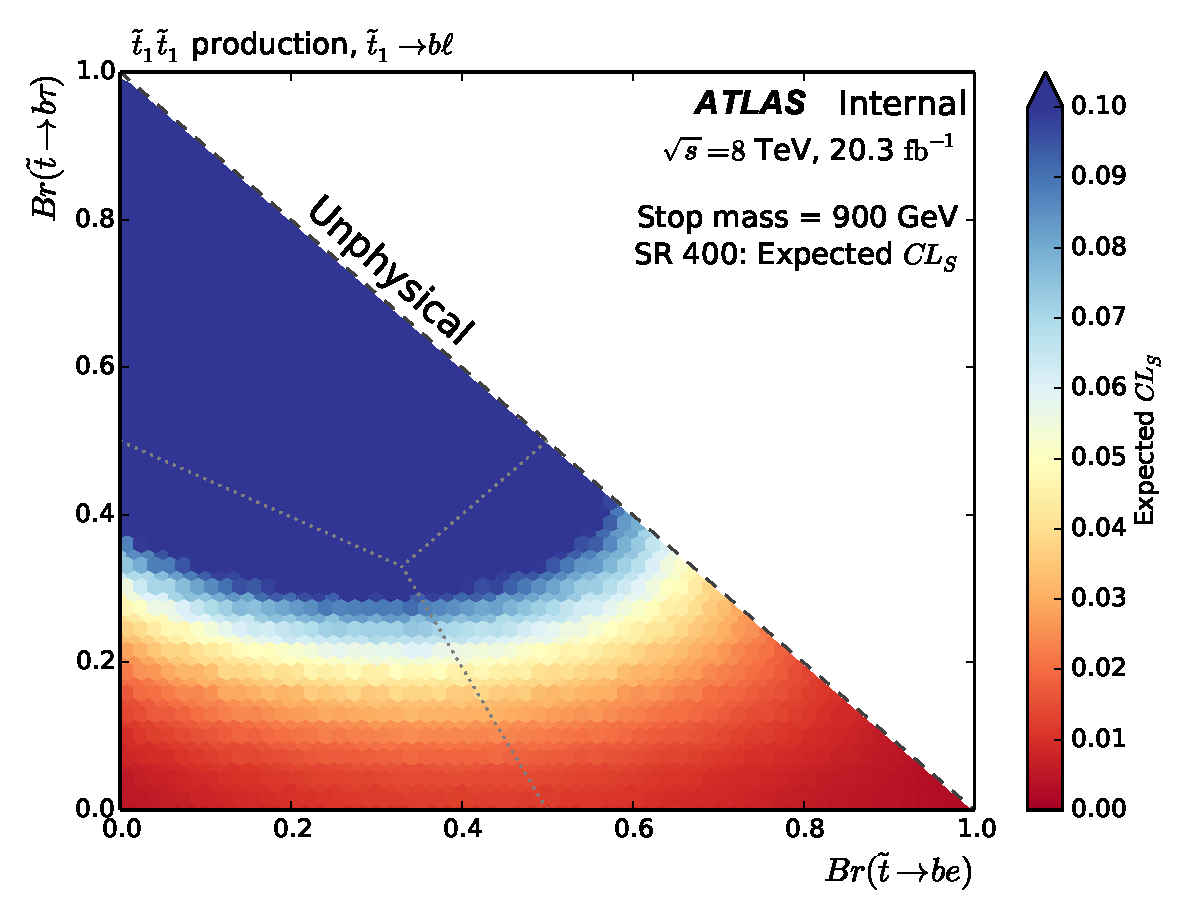
\includegraphics[width=0.65\textwidth]
      {figs/blstop/cls_plots/cls_vs_br_m_900_sr_400_exp.pdf}
  }
  \subbottom[Expected $CL_S$ or SR~600]{
    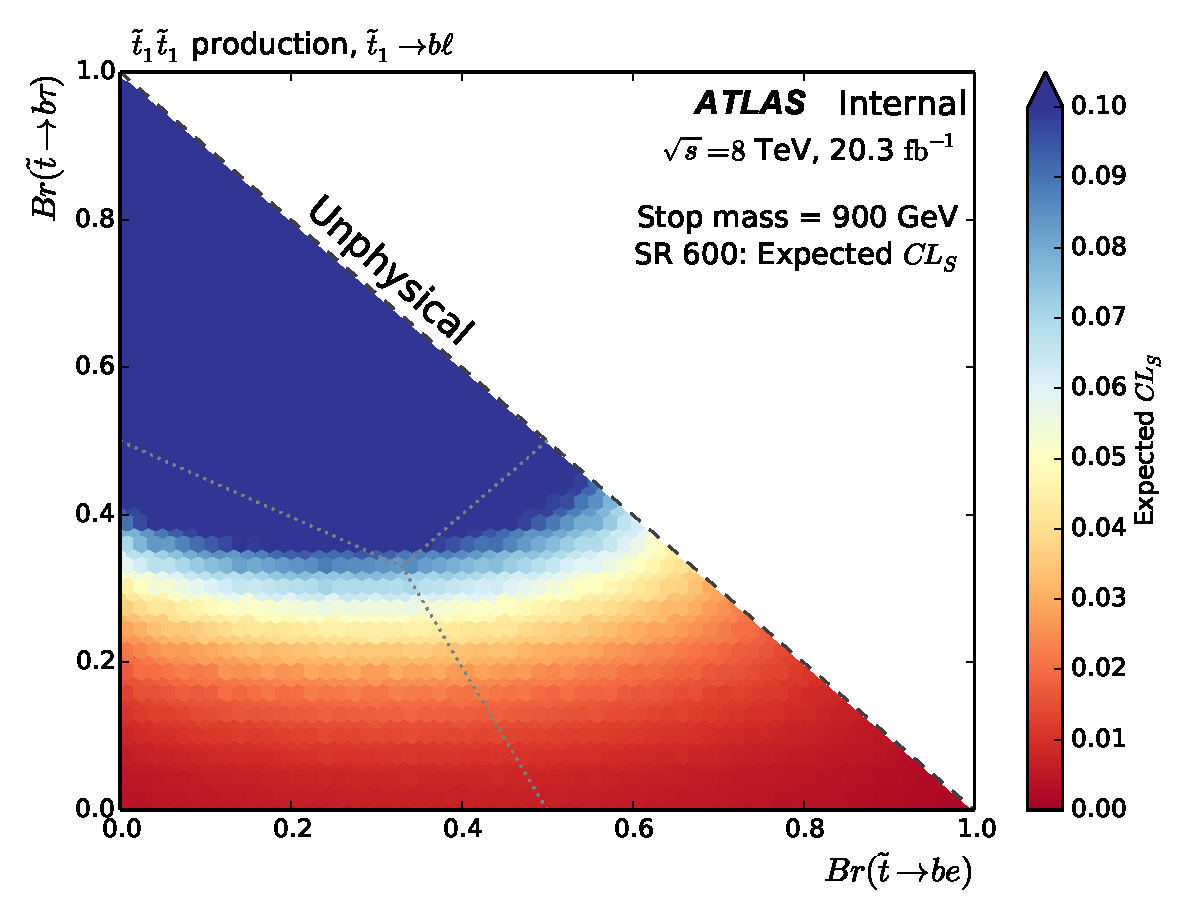
\includegraphics[width=0.65\textwidth]
      {figs/blstop/cls_plots/cls_vs_br_m_900_sr_600_exp.pdf}
  }
  \caption{
    Expected $CL_S$ values in SR~400 and SR~600 for a stop mass of 900~\GeV,
    shown across the plane of physical stop branching ratios.
  }
\end{figure}

\begin{figure}[ht]
  \centering
  \subbottom[Observed $CL_S$ or SR~400]{
    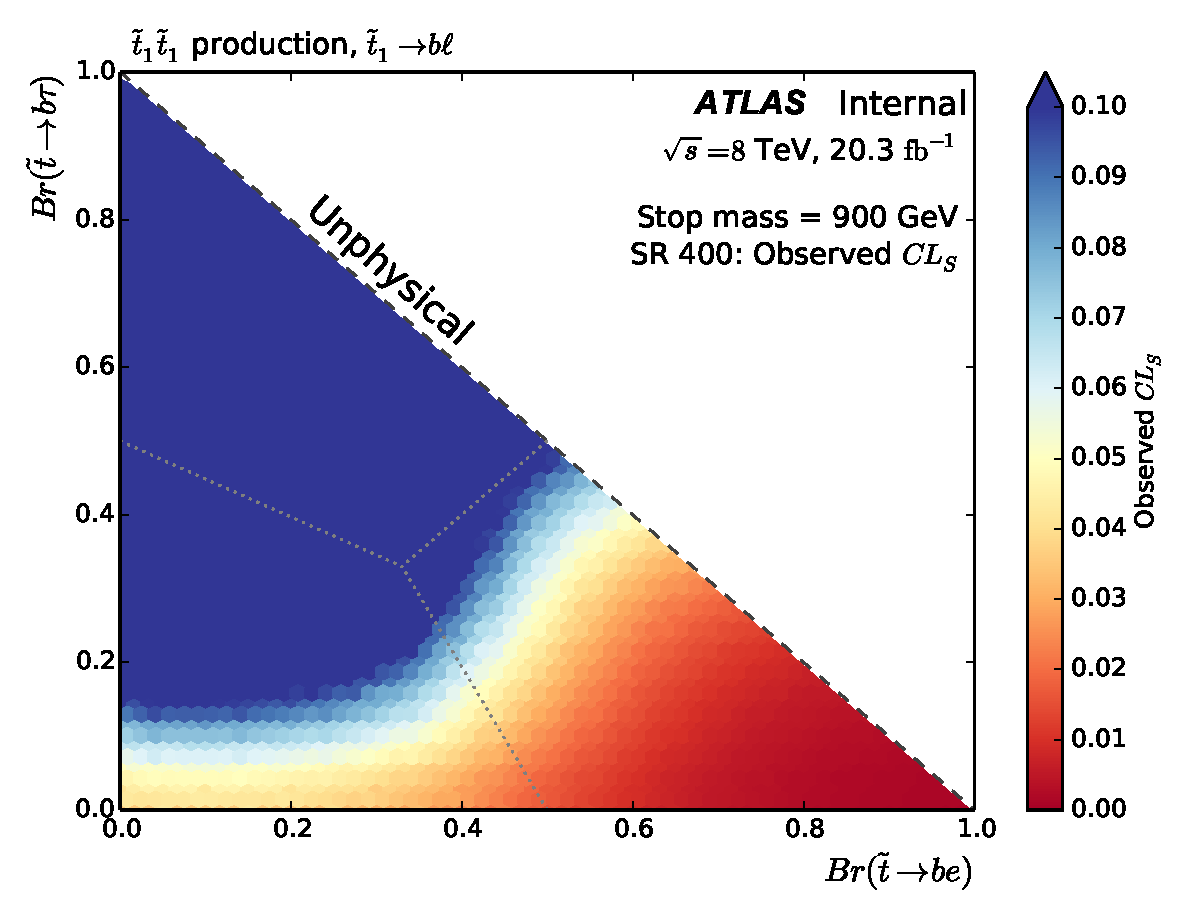
\includegraphics[width=0.65\textwidth]
      {figs/blstop/cls_plots/cls_vs_br_m_900_sr_400_obs.pdf}
  }
  \subbottom[Observed $CL_S$ or SR~600]{
    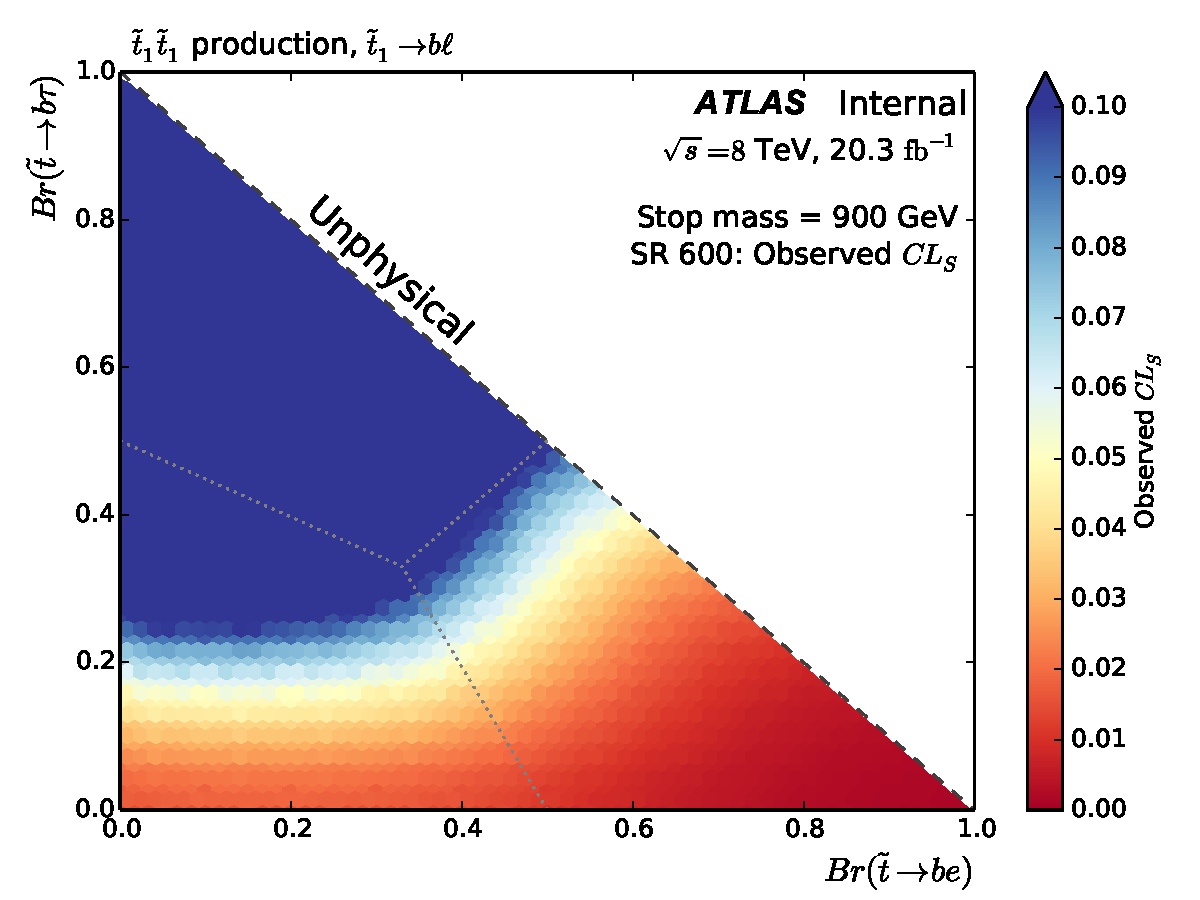
\includegraphics[width=0.65\textwidth]
      {figs/blstop/cls_plots/cls_vs_br_m_900_sr_600_obs.pdf}
  }
  \caption{
    Observed $CL_S$ values in SR~400 and SR~600 for a stop mass of 900~\GeV,
    shown across the plane of physical stop branching ratios.
  }
\end{figure}

\begin{figure}[ht]
  \centering
  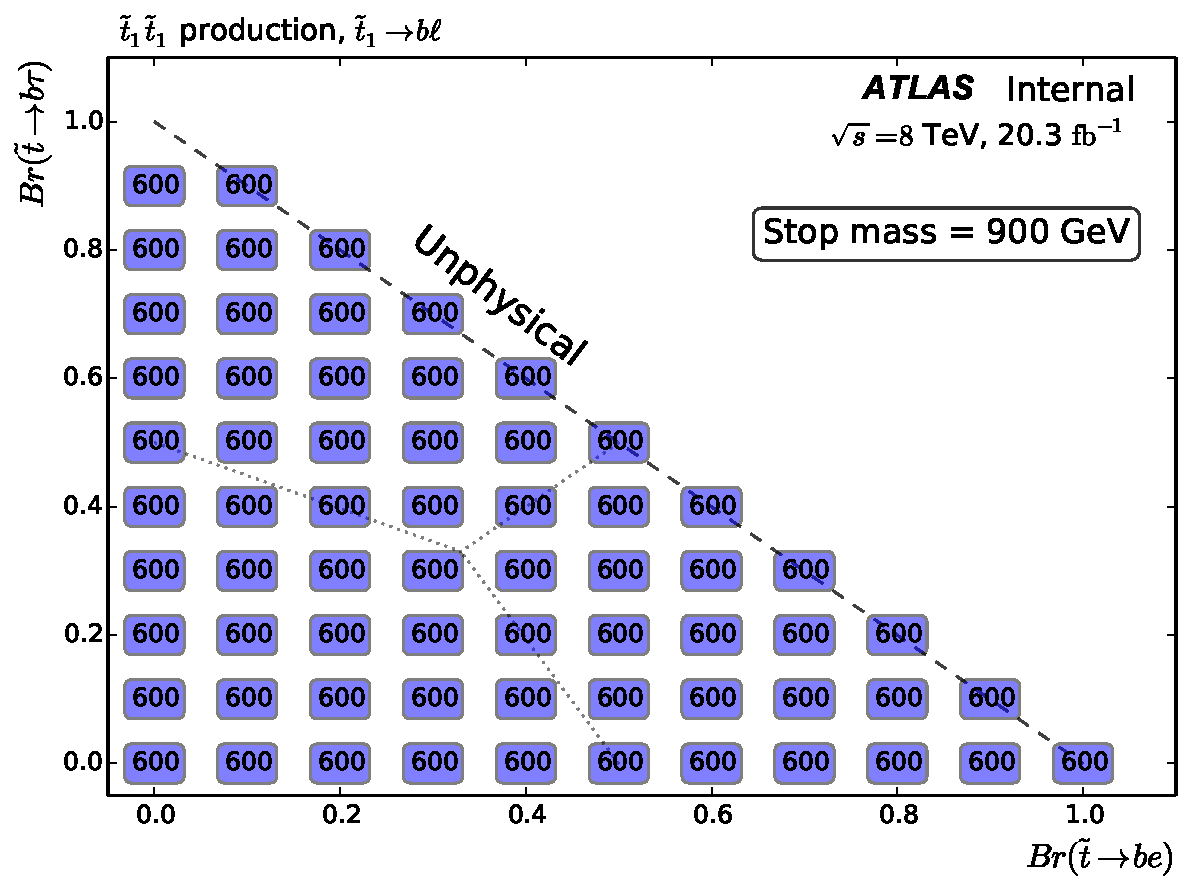
\includegraphics[width=0.65\textwidth]
    {figs/blstop/region_selection/region_choice_vs_br_m_900.pdf}
  \caption{
    Selected SR for select stop branching ratios for a stop mass of 900~\GeV.
    The SR is selected by choosing the SR with the smallest expected $CL_S$
    value for a given branching ratio.
    For several points in the branching ratio plane, SR~400 was selected because
    the two regions have the same expected $CL_S$ value, with the numerical
    precision of the statistical software.
    For these points, the expected sensitivity for both SRs is such that
    there is little difference between the expected sensitivity.
  }
\end{figure}

\FloatBarrier

%% -----------------------------------------------------------------------------
\newpage
\section{1000 \texorpdfstring{\GeV}{GeV} stop mass}

\begin{figure}[ht]
  \centering
  \subbottom[Expected $CL_S$ or SR~400]{
    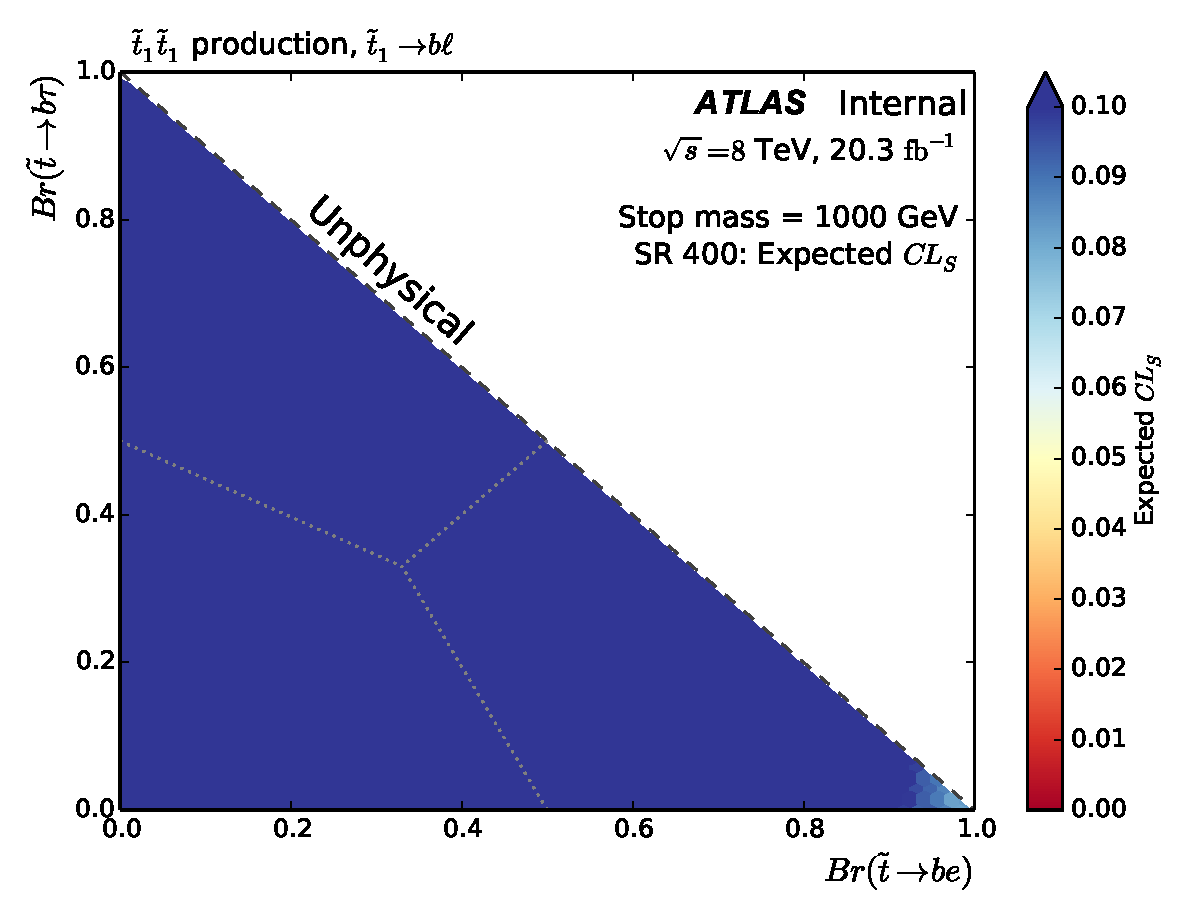
\includegraphics[width=0.65\textwidth]
      {figs/blstop/cls_plots/cls_vs_br_m_1000_sr_400_exp.pdf}
  }
  \subbottom[Expected $CL_S$ or SR~600]{
    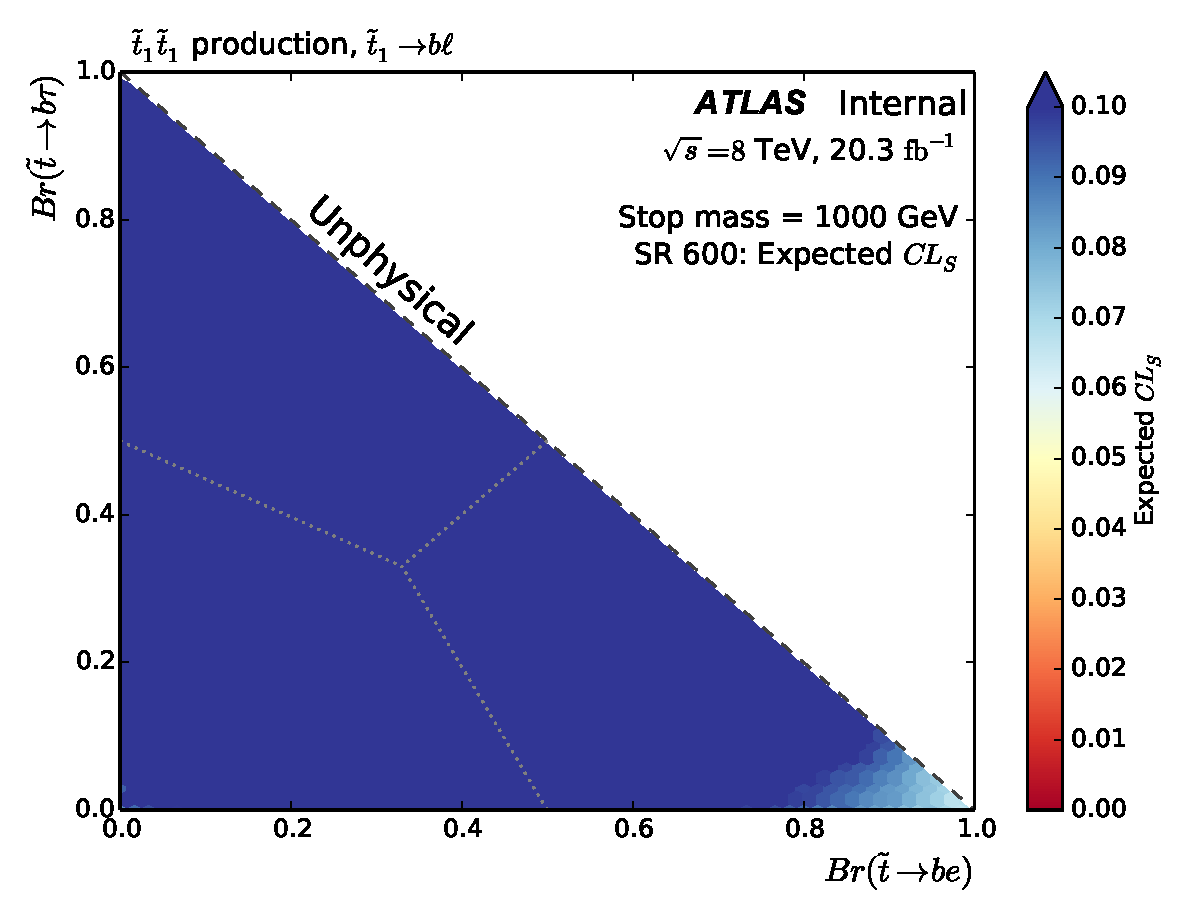
\includegraphics[width=0.65\textwidth]
      {figs/blstop/cls_plots/cls_vs_br_m_1000_sr_600_exp.pdf}
  }
  \caption{
    Expected $CL_S$ values in SR~400 and SR~600 for a stop mass of 1~\TeV,
    shown across the plane of physical stop branching ratios.
  }
\end{figure}

\begin{figure}[ht]
  \centering
  \subbottom[Observed $CL_S$ or SR~400]{
    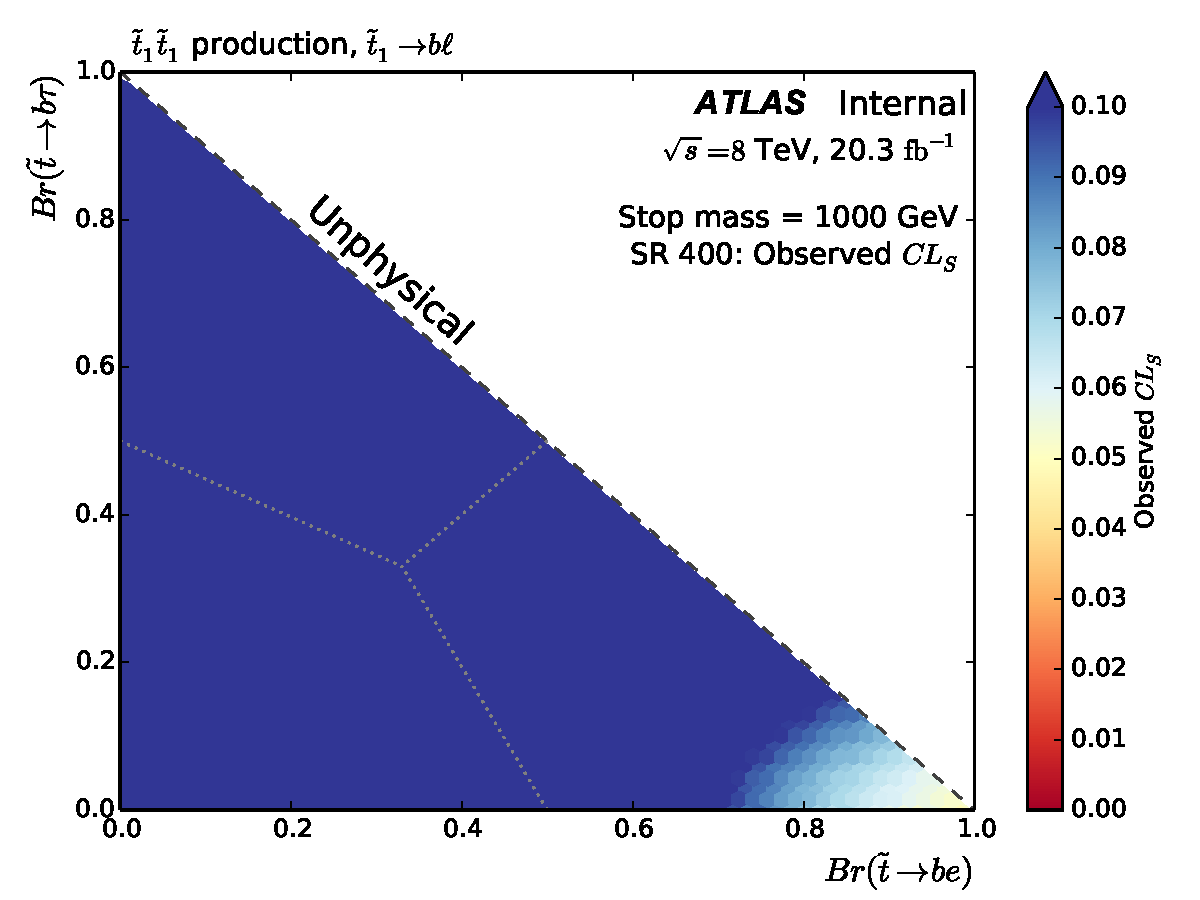
\includegraphics[width=0.65\textwidth]
      {figs/blstop/cls_plots/cls_vs_br_m_1000_sr_400_obs.pdf}
  }
  \subbottom[Observed $CL_S$ or SR~600]{
    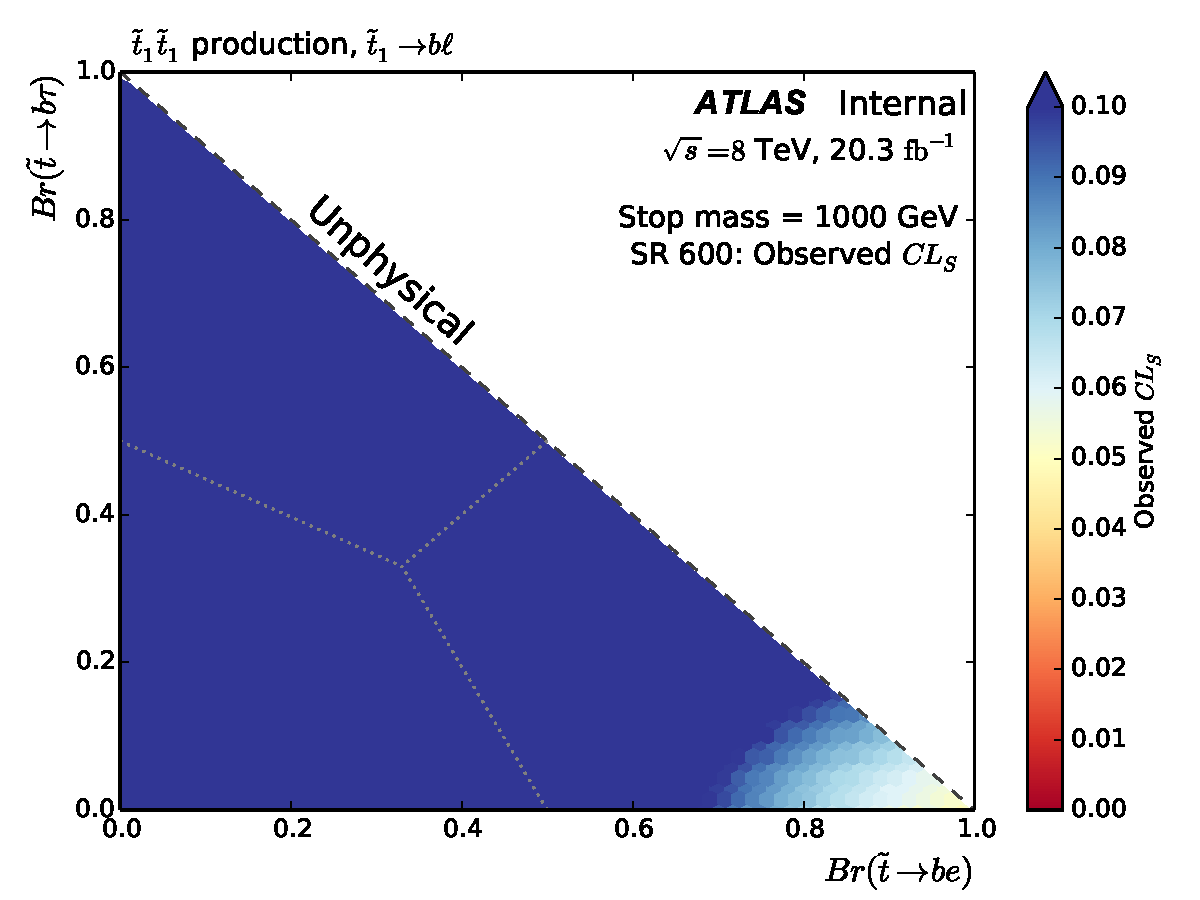
\includegraphics[width=0.65\textwidth]
      {figs/blstop/cls_plots/cls_vs_br_m_1000_sr_600_obs.pdf}
  }
  \caption{
    Observed $CL_S$ values in SR~400 and SR~600 for a stop mass of 1~\TeV,
    shown across the plane of physical stop branching ratios.
  }
\end{figure}

\begin{figure}[ht]
  \centering
  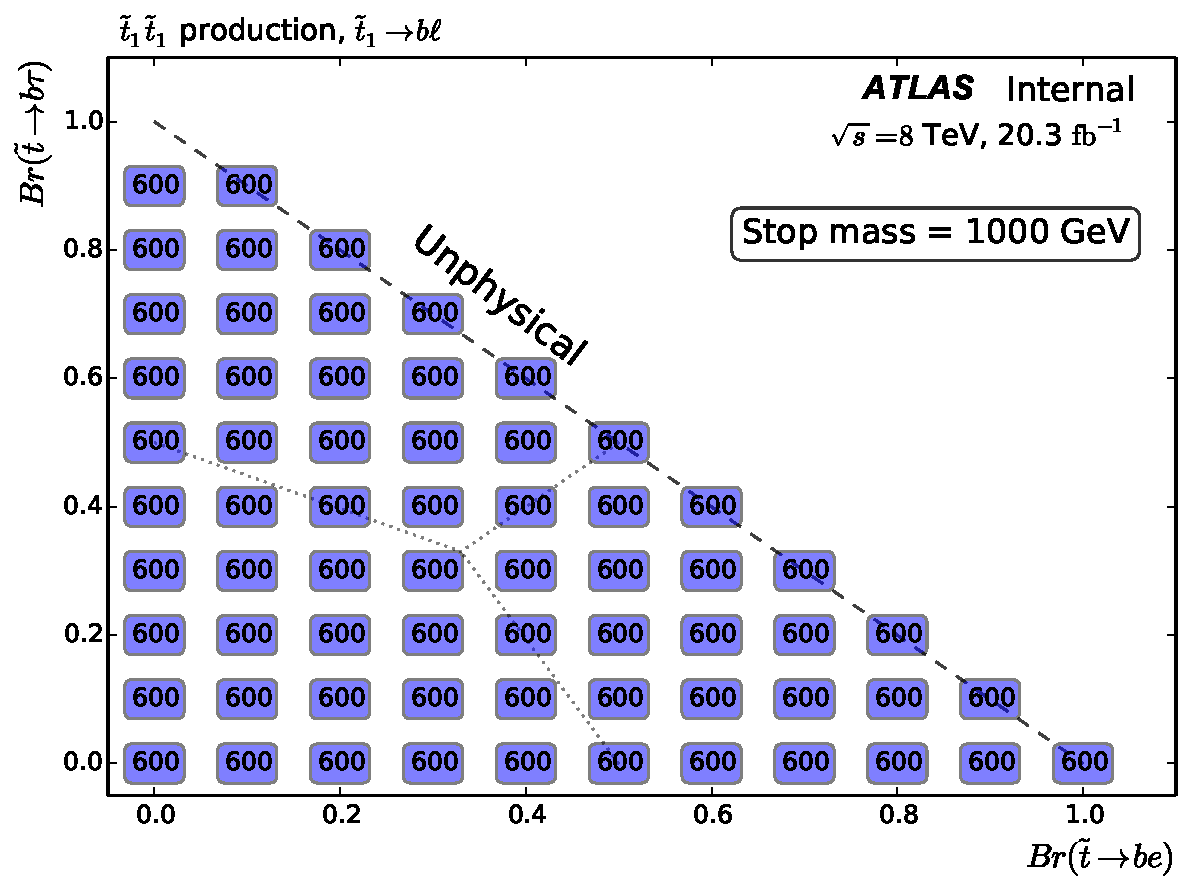
\includegraphics[width=0.65\textwidth]
    {figs/blstop/region_selection/region_choice_vs_br_m_1000.pdf}
  \caption{
    Selected SR for select stop branching ratios for a stop mass of 1~\TeV.
    The SR is selected by choosing the SR with the smallest expected $CL_S$
    value for a given branching ratio.
    For several points in the branching ratio plane, SR~400 was selected because
    the two regions have the same expected $CL_S$ value, with the numerical
    precision of the statistical software.
    For these points, the expected sensitivity for both SRs is such that
    there is little difference between the expected sensitivity.
  }
\end{figure}

\FloatBarrier

%% -----------------------------------------------------------------------------
\newpage
\section{1100 \texorpdfstring{\GeV}{GeV} stop mass}

\begin{figure}[ht]
  \centering
  \subbottom[Expected $CL_S$ or SR~400]{
    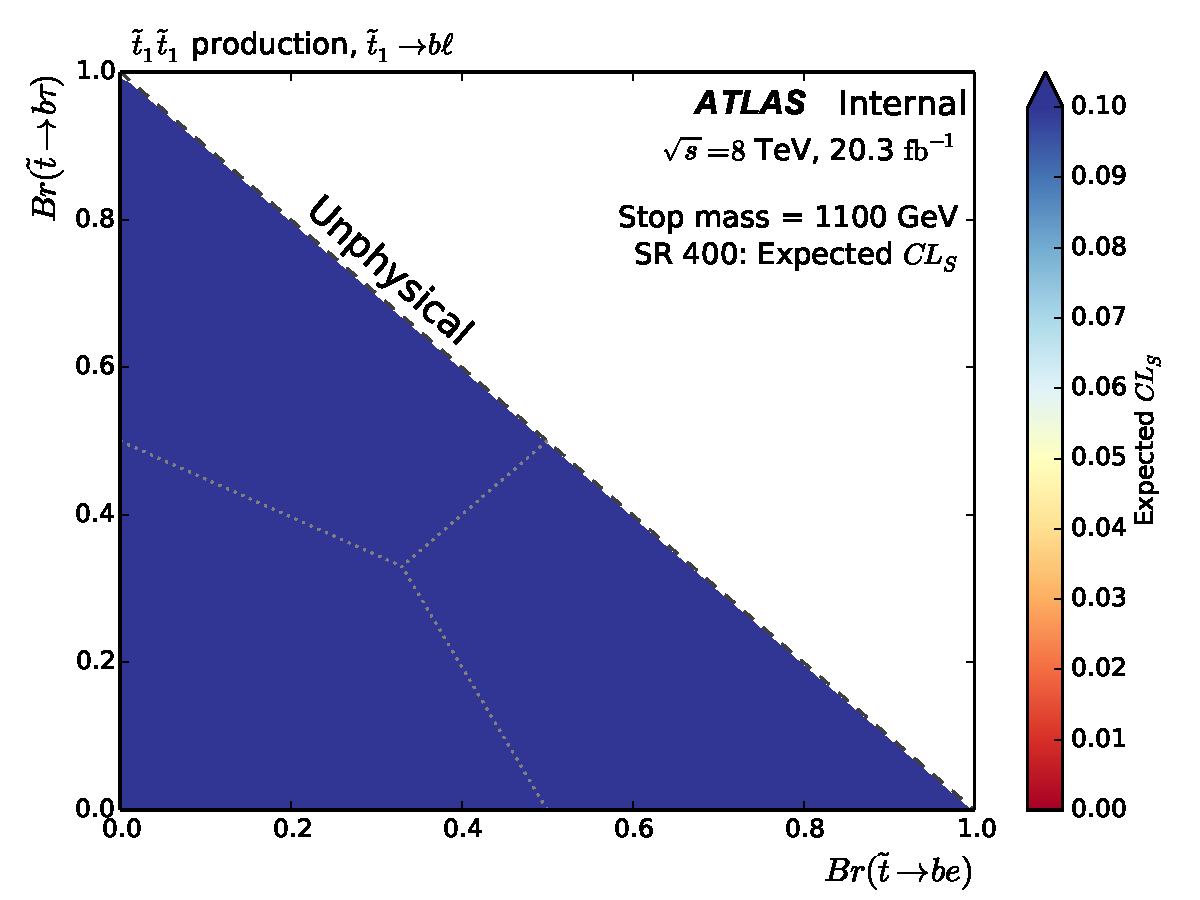
\includegraphics[width=0.65\textwidth]
      {figs/blstop/cls_plots/cls_vs_br_m_1100_sr_400_exp.pdf}
  }
  \subbottom[Expected $CL_S$ or SR~600]{
    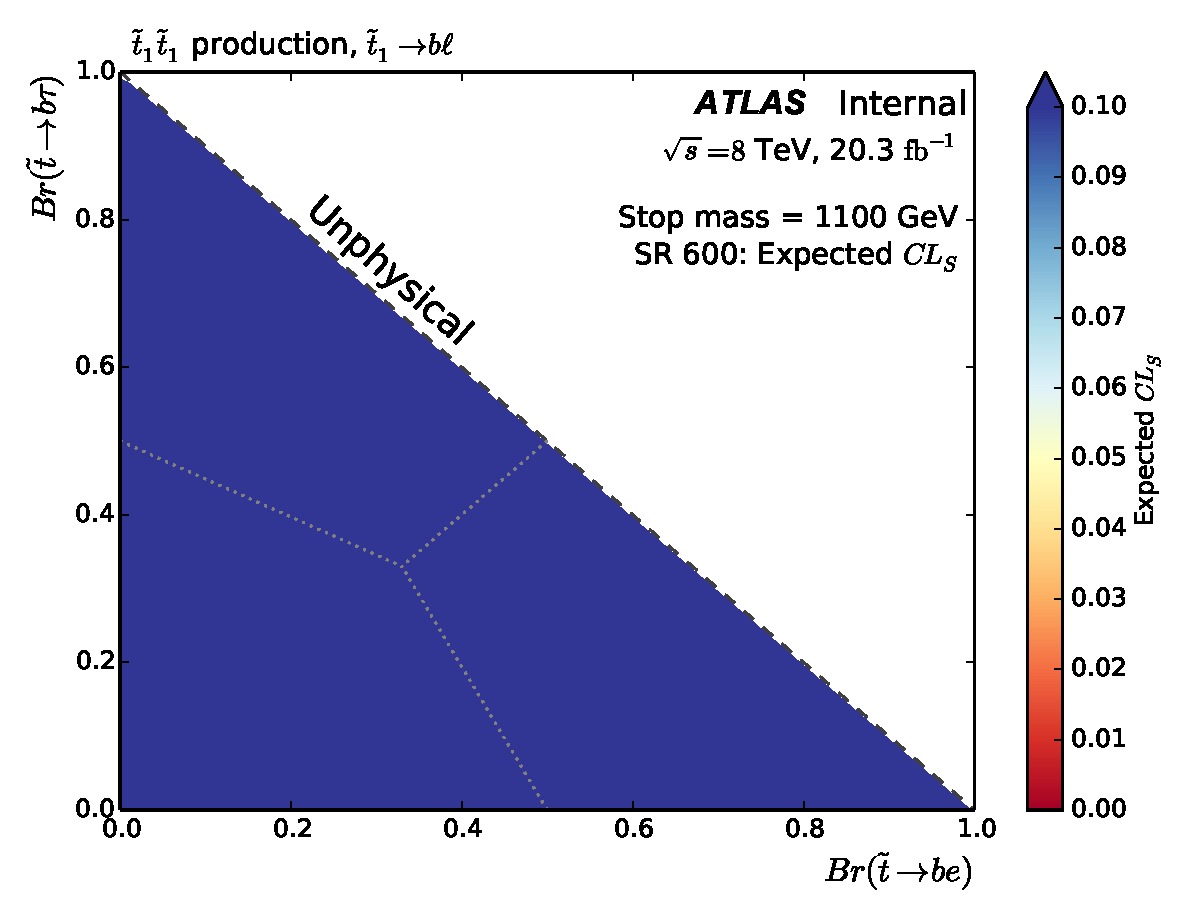
\includegraphics[width=0.65\textwidth]
      {figs/blstop/cls_plots/cls_vs_br_m_1100_sr_600_exp.pdf}
  }
  \caption{
    Expected $CL_S$ values in SR~400 and SR~600 for a stop mass of 1.1~\TeV,
    shown across the plane of physical stop branching ratios.
  }
\end{figure}

\begin{figure}[ht]
  \centering
  \subbottom[Observed $CL_S$ or SR~400]{
    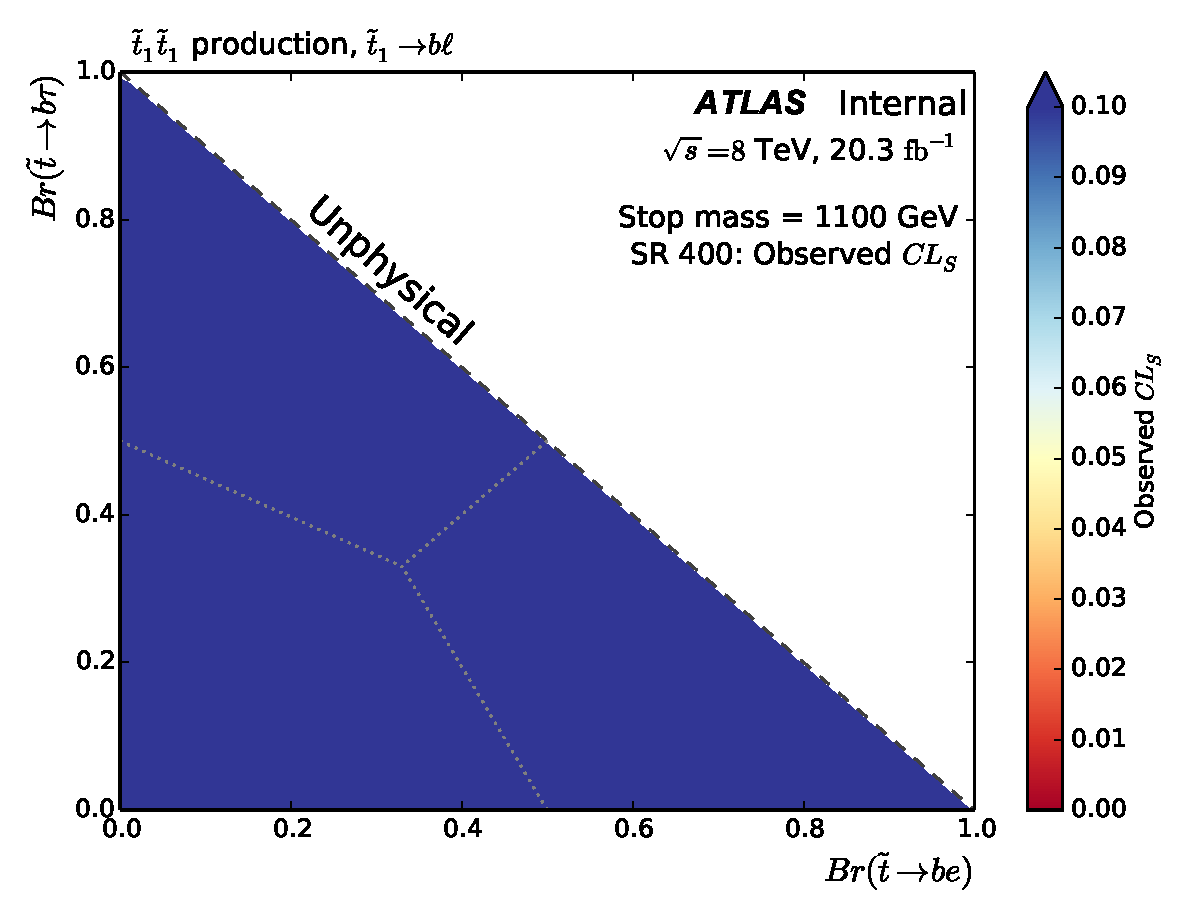
\includegraphics[width=0.65\textwidth]
      {figs/blstop/cls_plots/cls_vs_br_m_1100_sr_400_obs.pdf}
  }
  \subbottom[Observed $CL_S$ or SR~600]{
    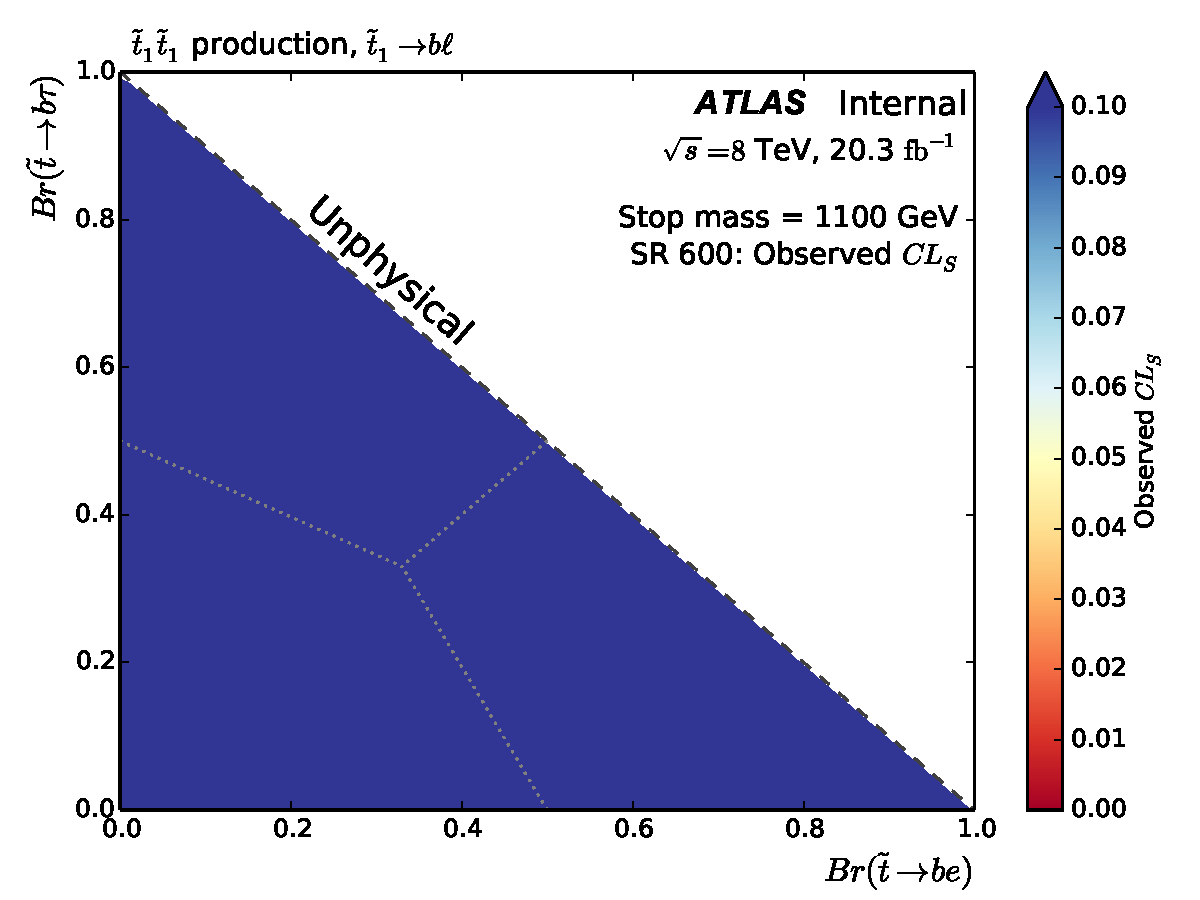
\includegraphics[width=0.65\textwidth]
      {figs/blstop/cls_plots/cls_vs_br_m_1100_sr_600_obs.pdf}
  }
  \caption{
    Observed $CL_S$ values in SR~400 and SR~600 for a stop mass of 1.1~\TeV,
    shown across the plane of physical stop branching ratios.
  }
\end{figure}

\begin{figure}[ht]
  \centering
  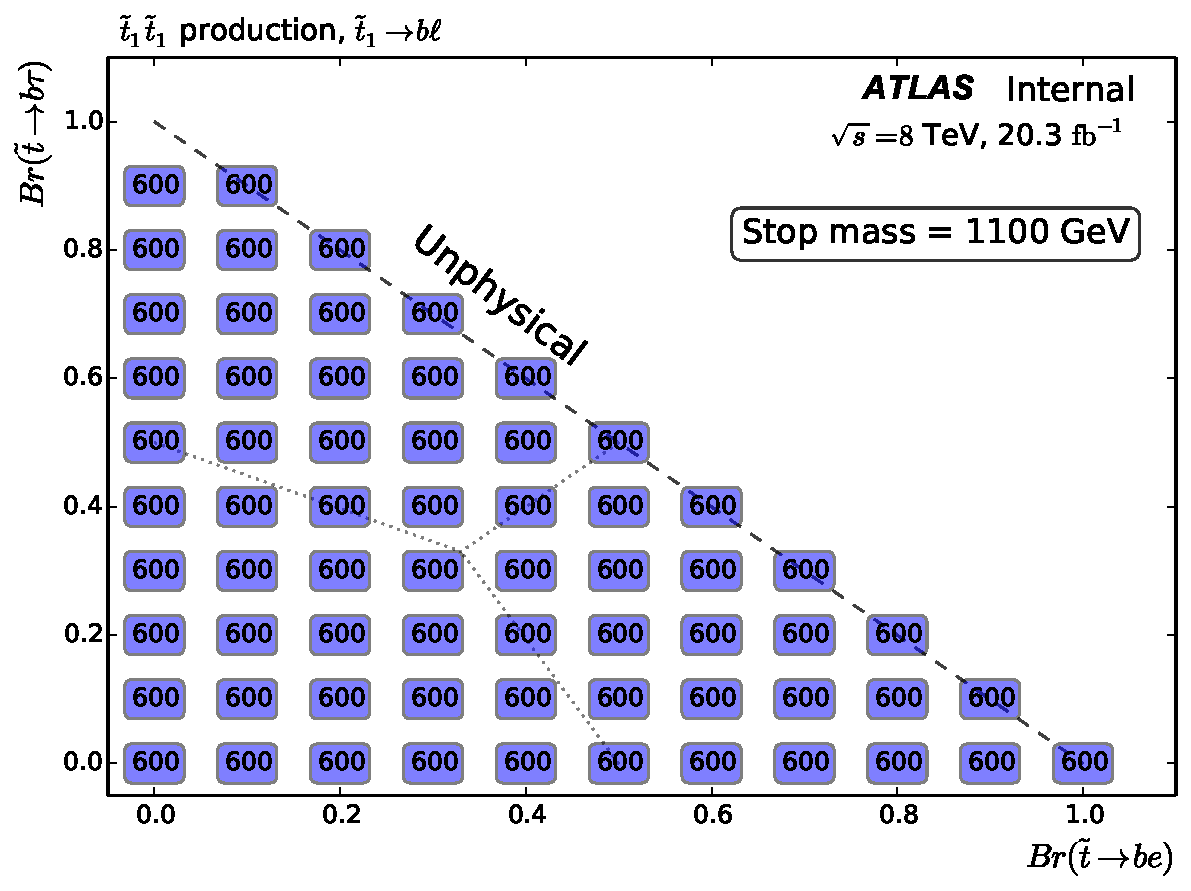
\includegraphics[width=0.65\textwidth]
    {figs/blstop/region_selection/region_choice_vs_br_m_1100.pdf}
  \caption{
    Selected SR for select stop branching ratios for a stop mass of 1.1~\TeV.
    The SR is selected by choosing the SR with the smallest expected $CL_S$
    value for a given branching ratio.
    For several points in the branching ratio plane, SR~400 was selected because
    the two regions have the same expected $CL_S$ value, with the numerical
    precision of the statistical software.
    For these points, the expected sensitivity for both SRs is such that
    there is little difference between the expected sensitivity.
  }
\end{figure}

\FloatBarrier

%% \begin{figure}[ht]
%%   \centering
%%   \subbottom[Expected $CL_S$ for SR 400]{
%%     \includegraphics[width=0.48\textwidth]
%%       {figs/blstop/cls_plots/cls_vs_br_m_400_sr_400_exp.pdf}}
%%   \subbottom[Expected $CL_S$ for SR 600]{
%%     \includegraphics[width=0.48\textwidth]
%%       {figs/blstop/cls_plots/cls_vs_br_m_400_sr_600_exp.pdf}}
%%   % \subbottom[Selected region]{
%%   %   \includegraphics[width=0.48\textwidth]
%%   %     {figs/blstop/region_selection/region_choice_vs_br_m_400.pdf}}
%%   \caption{blah blah blah expected blah blah blah}
%% \end{figure}

% \begin{figure}[ht]
%   \centering
%   \subbottom[Observed $CL_S$ for SR 400]{
%     \includegraphics[width=0.40\textwidth]
%       {figs/blstop/cls_plots/cls_vs_br_m_400_sr_400_obs.pdf}}
%   \subbottom[Observed $CL_S$ for SR 600]{
%     \includegraphics[width=0.40\textwidth]
%       {figs/blstop/cls_plots/cls_vs_br_m_400_sr_600_obs.pdf}}
%   \caption{blah blah blah observed blah blah blah}
% \end{figure}

% \FloatBarrier


%% figs/blstop/cls_plots/cls_vs_br_m_500_sr_400_exp.pdf
%% figs/blstop/cls_plots/cls_vs_br_m_500_sr_400_obs.pdf
%% figs/blstop/cls_plots/cls_vs_br_m_500_sr_600_exp.pdf
%% figs/blstop/cls_plots/cls_vs_br_m_500_sr_600_obs.pdf
%% figs/blstop/cls_plots/cls_vs_br_m_600_sr_400_exp.pdf
%% figs/blstop/cls_plots/cls_vs_br_m_600_sr_400_obs.pdf
%% figs/blstop/cls_plots/cls_vs_br_m_600_sr_600_exp.pdf
%% figs/blstop/cls_plots/cls_vs_br_m_600_sr_600_obs.pdf
%% figs/blstop/cls_plots/cls_vs_br_m_700_sr_400_exp.pdf
%% figs/blstop/cls_plots/cls_vs_br_m_700_sr_400_obs.pdf
%% figs/blstop/cls_plots/cls_vs_br_m_700_sr_600_exp.pdf
%% figs/blstop/cls_plots/cls_vs_br_m_700_sr_600_obs.pdf
%% figs/blstop/cls_plots/cls_vs_br_m_800_sr_400_exp.pdf
%% figs/blstop/cls_plots/cls_vs_br_m_800_sr_400_obs.pdf
%% figs/blstop/cls_plots/cls_vs_br_m_800_sr_600_exp.pdf
%% figs/blstop/cls_plots/cls_vs_br_m_800_sr_600_obs.pdf
%% figs/blstop/cls_plots/cls_vs_br_m_900_sr_400_exp.pdf
%% figs/blstop/cls_plots/cls_vs_br_m_900_sr_400_obs.pdf
%% figs/blstop/cls_plots/cls_vs_br_m_900_sr_600_exp.pdf
%% figs/blstop/cls_plots/cls_vs_br_m_900_sr_600_obs.pdf
%% 
%% figs/blstop/cls_plots/cls_vs_br_m_1000_sr_400_exp.pdf
%% figs/blstop/cls_plots/cls_vs_br_m_1000_sr_400_obs.pdf
%% figs/blstop/cls_plots/cls_vs_br_m_1000_sr_600_exp.pdf
%% figs/blstop/cls_plots/cls_vs_br_m_1000_sr_600_obs.pdf
%% figs/blstop/cls_plots/cls_vs_br_m_1100_sr_400_exp.pdf
%% figs/blstop/cls_plots/cls_vs_br_m_1100_sr_400_obs.pdf
%% figs/blstop/cls_plots/cls_vs_br_m_1100_sr_600_exp.pdf
%% figs/blstop/cls_plots/cls_vs_br_m_1100_sr_600_obs.pdf
%% 
%% figs/blstop/region_selection/region_choice_vs_br_m_500.pdf
%% figs/blstop/region_selection/region_choice_vs_br_m_600.pdf
%% figs/blstop/region_selection/region_choice_vs_br_m_700.pdf
%% figs/blstop/region_selection/region_choice_vs_br_m_800.pdf
%% figs/blstop/region_selection/region_choice_vs_br_m_900.pdf
%% figs/blstop/region_selection/region_choice_vs_br_m_1000.pdf
%% figs/blstop/region_selection/region_choice_vs_br_m_1100.pdf
